\clearpage

\subsection{Scale factors}
\label{sec:scale-factors}

In Section~\ref{sec:object-selection-electrons} and Section~\ref{sec:muon-selection}, the selection applied to electrons and muons respectively was studied, and a choice was made regarding the identification working point. Simulation was exclusively used to draw conclusions about the identification efficiency of the leptons. However, relying solely on \gls{mc} simulation can produce significant systematic errors due to imperfections in modeling both the data and the detector response. Therefore, measuring the identification efficiency in data is necessary to correct any potentially false efficiency rates in the simulation. The term \emph{efficiency} refers to the probability of reconstructing or identifying a lepton. For a lepton $\ell$, the identification efficiency is defined as:

\begin{equation}
\varepsilon_{\ell}^{\mathrm{ID}} = \frac{N_{\ell}(\mathrm{ID})}{N_{\ell}(\mathrm{produced})}
\end{equation}

In \gls{mc} simulation, the number of produced leptons is the same as the number of generated leptons. However, in data, the efficiency must be measured using a data-driven method. Once the efficiencies have been measured both in simulation and data, a correction factor called the \gls{sf} can be applied to the simulation to correct any discrepancies that may arise. Scale factors are defined as the ratio between the efficiency in data and the efficiency in simulation:

\begin{equation}
\mathrm{SF}_{\ell}^{\mathrm{ID}}=\frac{\varepsilon_{\ell}^{\mathrm{ID,Data}}}{\varepsilon_{\ell}^{\mathrm{ID,MC}}},
\end{equation}

dropping the superscript ID, this becomes:

\begin{equation}
\mathrm{SF}_{\ell}=\frac{\varepsilon_{\ell}^{\mathrm{Data}}}{\varepsilon_{\ell}^{\mathrm{MC}}}.
\end{equation}

Once the relevant \gls{sf} have been determined, they are applied to every lepton that passes the object selection in the event. The scale factors for loose-ID electrons in the relevant \pt range have been centrally measured by the corresponding working group and are applied to the selected electrons. As determined in Section~\ref{sec:muon-selection}, the analysis signal muon's lower \pt threshold is $2\GeV$, which is low. Scale factors for medium ID leptons with $\pt\geq 2\GeV$ were computed centrally by the Muon \gls{pog}. However, the scale factors were computed by requiring $\DR > 0.5$ between the muons, as mentioned in~\cite{muon-id-sf-2016,muon-id-sf-2016-pres}, and while they match the muons' \pt range and identification working point, $\DR < 0.5$ is one of the drivers of sensitivity, as seen in Section~\ref{sec:lepton-dr}. Therefore, it is necessary to validate the scale factors in that region and show that the efficiencies have no $\DR$ dependence. To do so, the efficiencies in different $\DR$ regions are calculated.

In order to measure such efficiencies in data, one must identify desired leptons with low and easily reducible fakes. A widely used method to perform such a data-driven task is the Tag \& Probe method. This involves examining a mass resonance such as \PZ, \JPsi or \PGU to select particles of the desired type, and probing the efficiency of a particular selection criterion on those particles. The mass resonance then decays into two same-flavor opposite charged pairs of leptons, forming a peak on top of a background. To measure the efficiency of low \pt muons, dimuon events around the \JPsi mass window are chosen. One muon is labeled as a `tag' and the other as a `probe'. The tag muon is selected with a very tight selection resulting in high certainty that the object corresponds to a real produced muon. The probe is given a loose selection but constrained to be consistent with a product of a \JPsi, almost certainly originating from a real muon as well. The background is easily removed by fitting the shape of the \JPsi. The probe is then subjected to cuts or constraints, used to measure a particular efficiency. This study aims to show that the efficiency to identify a muon with a medium ID working point from a track has no $\DR$ dependence. Therefore, the efficiency in question is defined as:

\begin{equation}
\varepsilon_{\mu}^{\mathrm{ID}} = \frac{N_{\mu}^\mathrm{ID}}{N_{t}}.
\end{equation}

The denominator probe used in the study refers to a track that has passed a loose selection, while the numerator probe track is required to match a medium ID working point muon. To determine the number of objects passing a selection, a fit is performed on data and \gls{mc} samples to measure the corresponding efficiencies.

This study was conducted for the year 2016. The 2016 samples listed in Section~\ref{sec:sm-mc} are used for \gls{mc}. To ensure the independence of the tagged muon from the triggered object, a single electron trigger is used for data. The corresponding data set is measured to be 36.02\fbinv using the BRIL Work Suite~\cite{bril}. The following trigger paths are utilized:

\begin{itemize}
\item \texttt{HLT\_Ele27\_WPTight\_Gsf\_v*},
\item \texttt{HLT\_Ele27\_eta2p1\_WPLoose\_Gsf\_v*},
\item \texttt{HLT\_Ele32\_WPTight\_Gsf\_v*},
\item \texttt{HLT\_Ele35\_WPTight\_Gsf\_v*}.
\end{itemize}

An offline loose ID electron with $\pt>27\GeV$ is then selected. The requirements to select a tag \& probe pair are defined in Table~\ref{tab:tag-probe-def}.

\begin{table}[!htb]
	\centering
	\label{tab:tag-probe-def}
		\caption{Selection criteria for Tags and Probes}
		%\vspace{1mm}
			\begin{tabular}{l|l} \hline
			Tag & Probe \\ \hline
			medium ID muon & isolated track\\
			$\pt \geq 5\GeV$ & $2\leq\pt\leq 20\GeV$  ($ \pt\geq 3 \GeV $ for barrel) \\
			$\abs{\eta}<2.4$ & opposite-sign in invariant mass window $[2.5,3.5]\GeV$ \\ \hline
			\end{tabular}
\end{table}

A fit is then performed in an invariant mass window around the \JPsi peak of $[2.5,3.5]\GeV$. The signal fit uses a crystal ball function, and the continuum is fit with a 6th order polynomial. The fit is repeated twice, where the denominator is based on probe tracks, and the numerator uses medium ID muons that have been matched to those tracks. The \DR range has been split into three, and the $\abs{\eta}$ of the muons has been divided into barrel ($\abs{\eta}<1.2$) and endcaps ($1.2<\abs{\eta}<2.4$). Simulation fits are shown in Figure~\ref{fig:tb-barrel-simulation} for the barrel, and Figure~\ref{fig:tb-endcaps-simulation} for the endcaps. Data fits are shown in Figure~\ref{fig:tb-barrel-data} for the barrel, and in Figure~\ref{fig:tb-endcaps-data} for the endcaps.

\begin{figure}[!htbp]
\centering
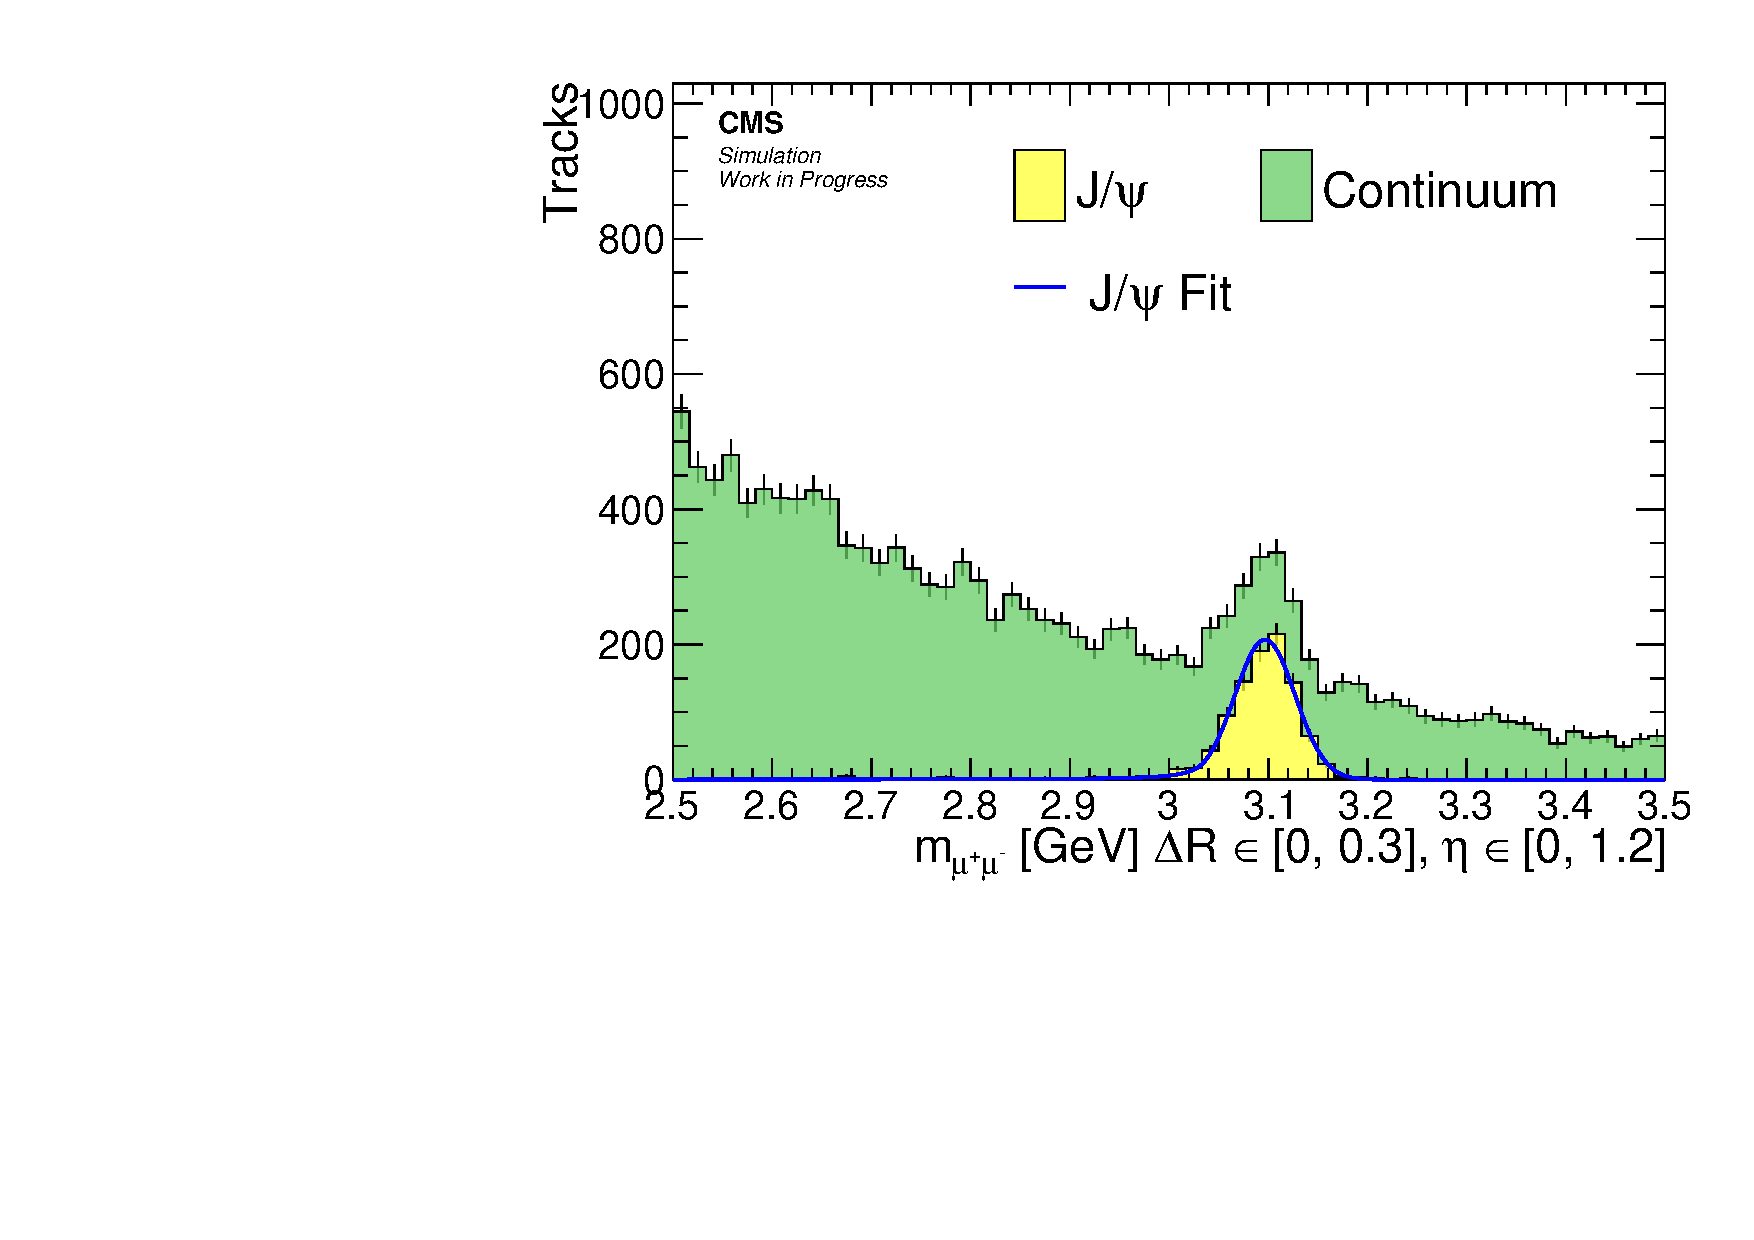
\includegraphics[width=0.32\linewidth]{plots/jpsi_muons_fit_bg_delta_r_single_electron/none_invMass_0_0.3_0_1.2.pdf} \,
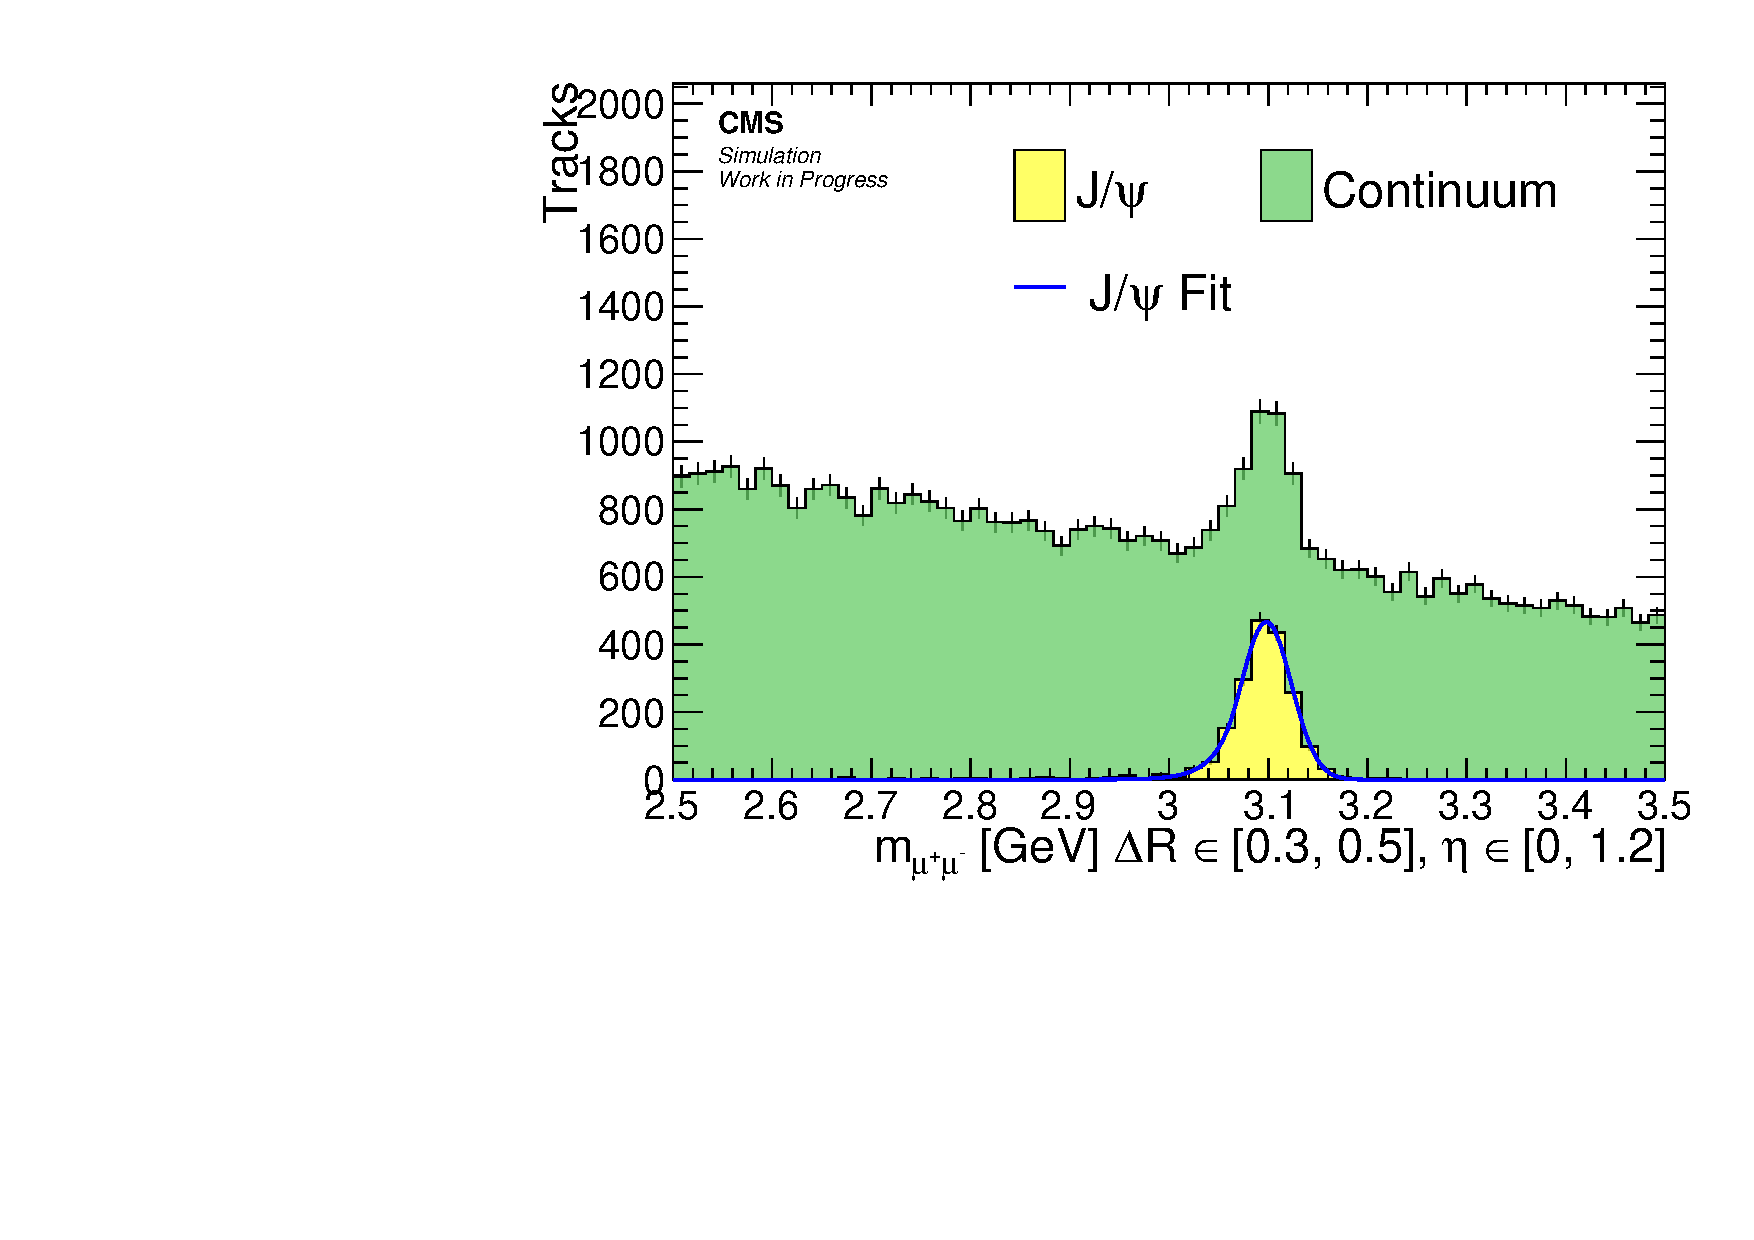
\includegraphics[width=0.32\linewidth]{plots/jpsi_muons_fit_bg_delta_r_single_electron/none_invMass_0.3_0.5_0_1.2.pdf}  \,
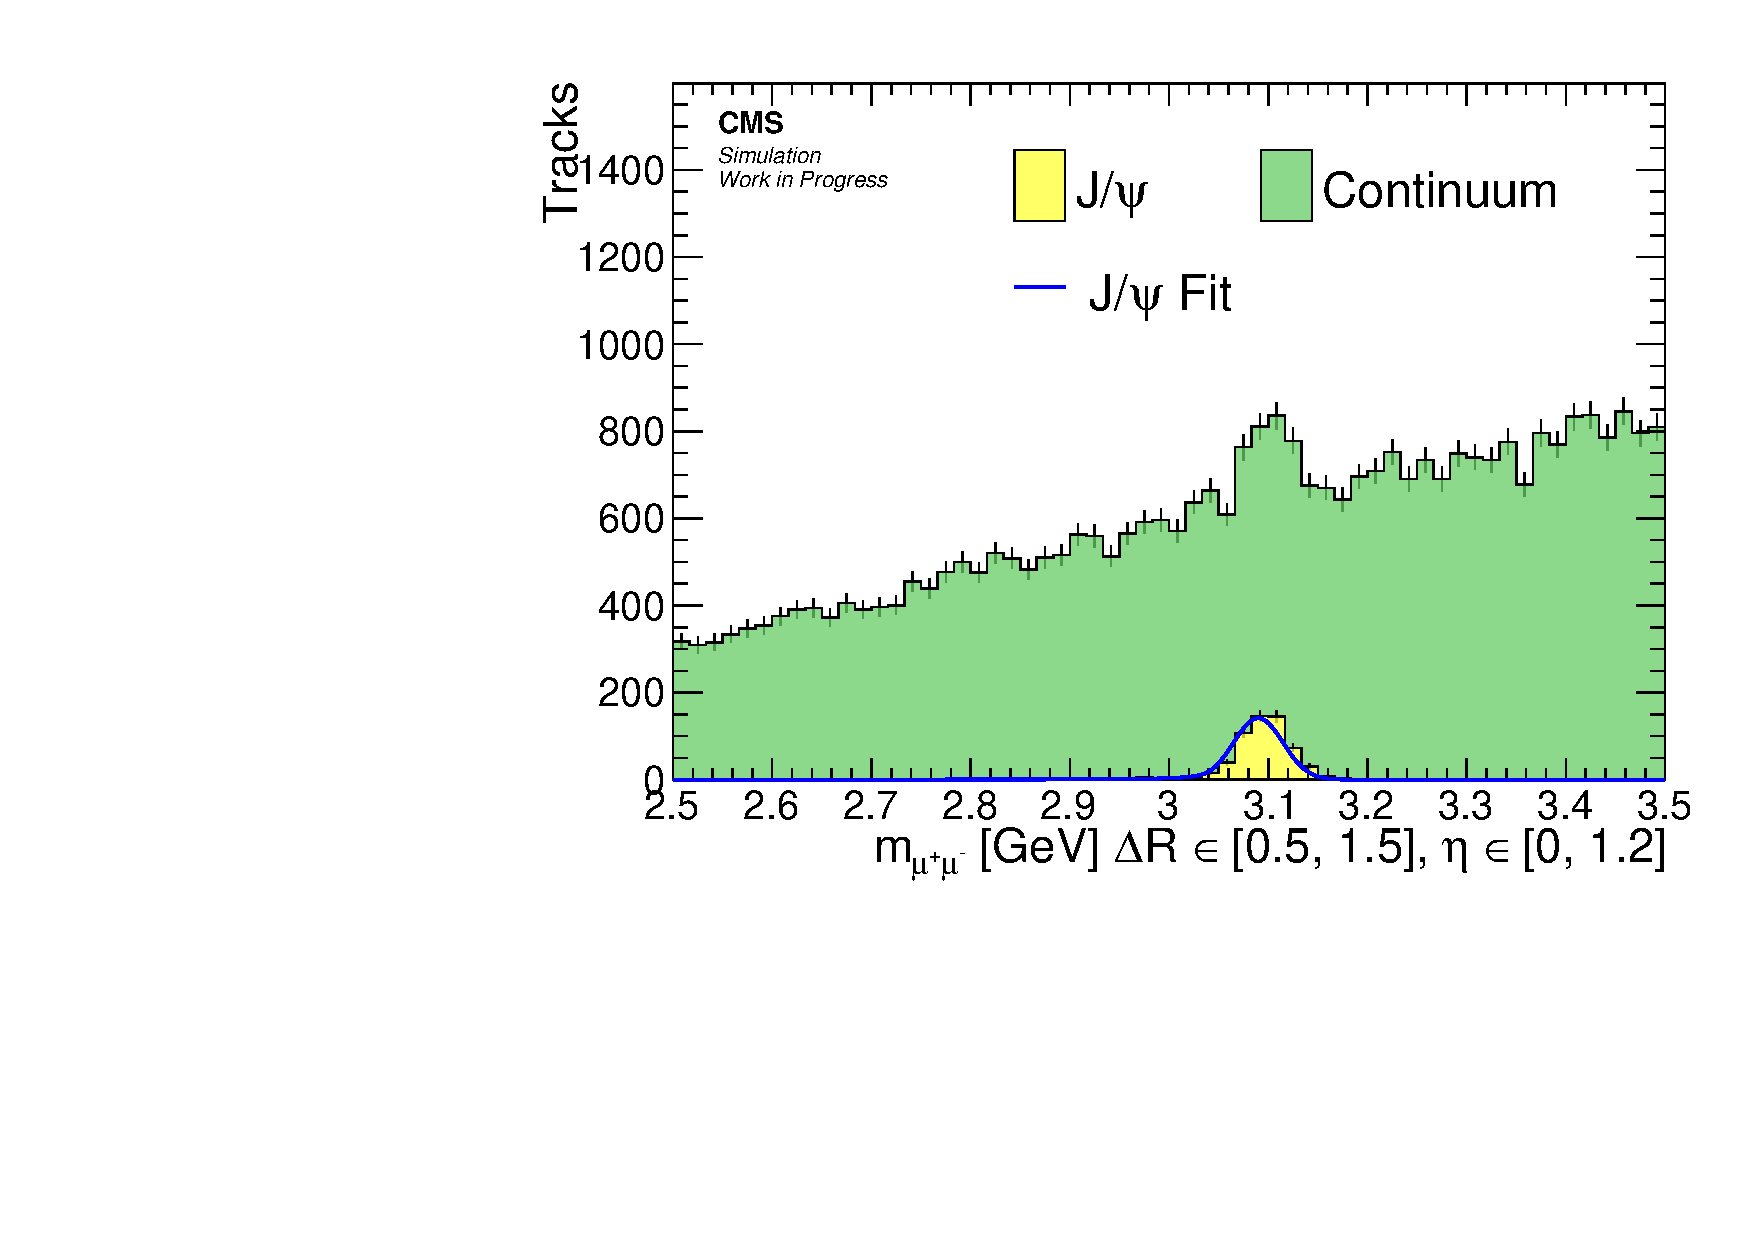
\includegraphics[width=0.32\linewidth]{plots/jpsi_muons_fit_bg_delta_r_single_electron/none_invMass_0.5_1.5_0_1.2.pdf} \\
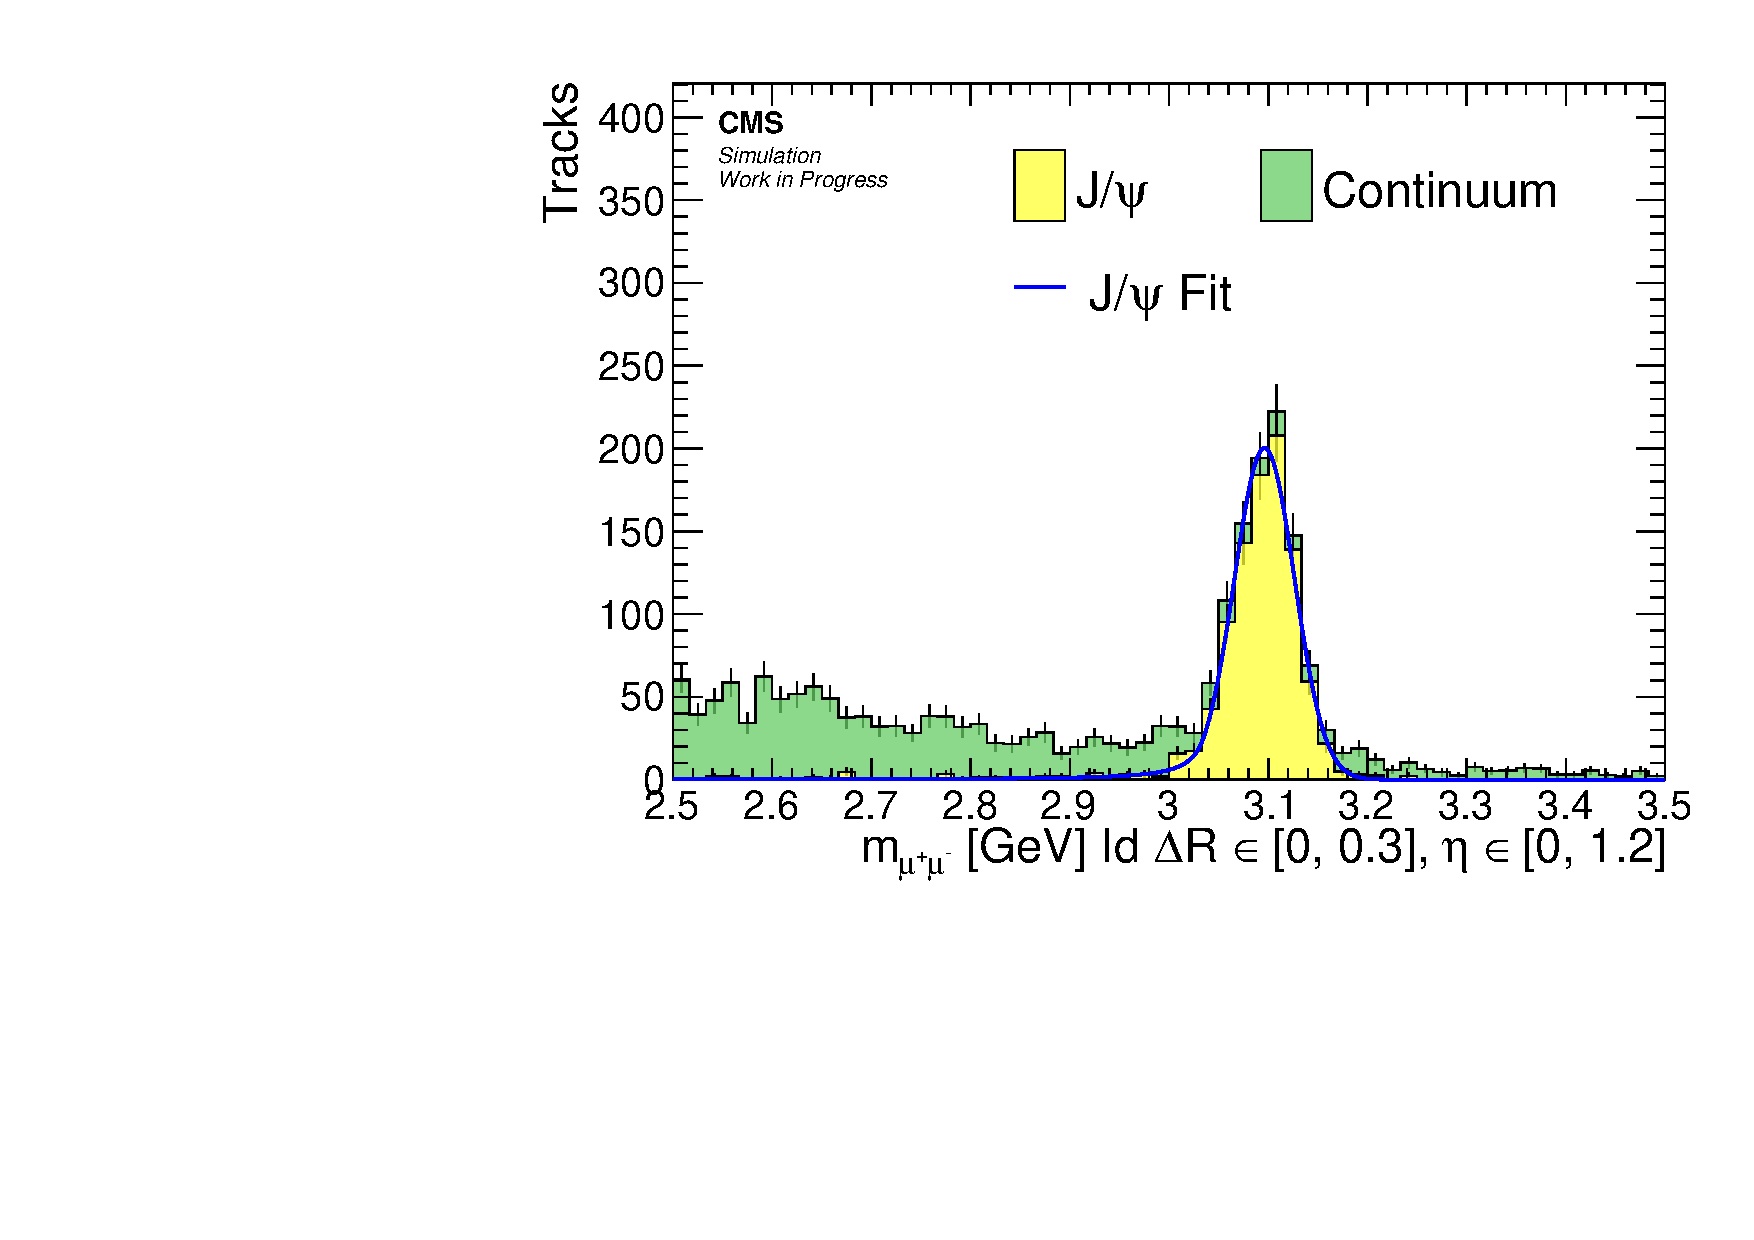
\includegraphics[width=0.32\linewidth]{plots/jpsi_muons_fit_bg_delta_r_single_electron/none_id_invMass_0_0.3_0_1.2.pdf} \,
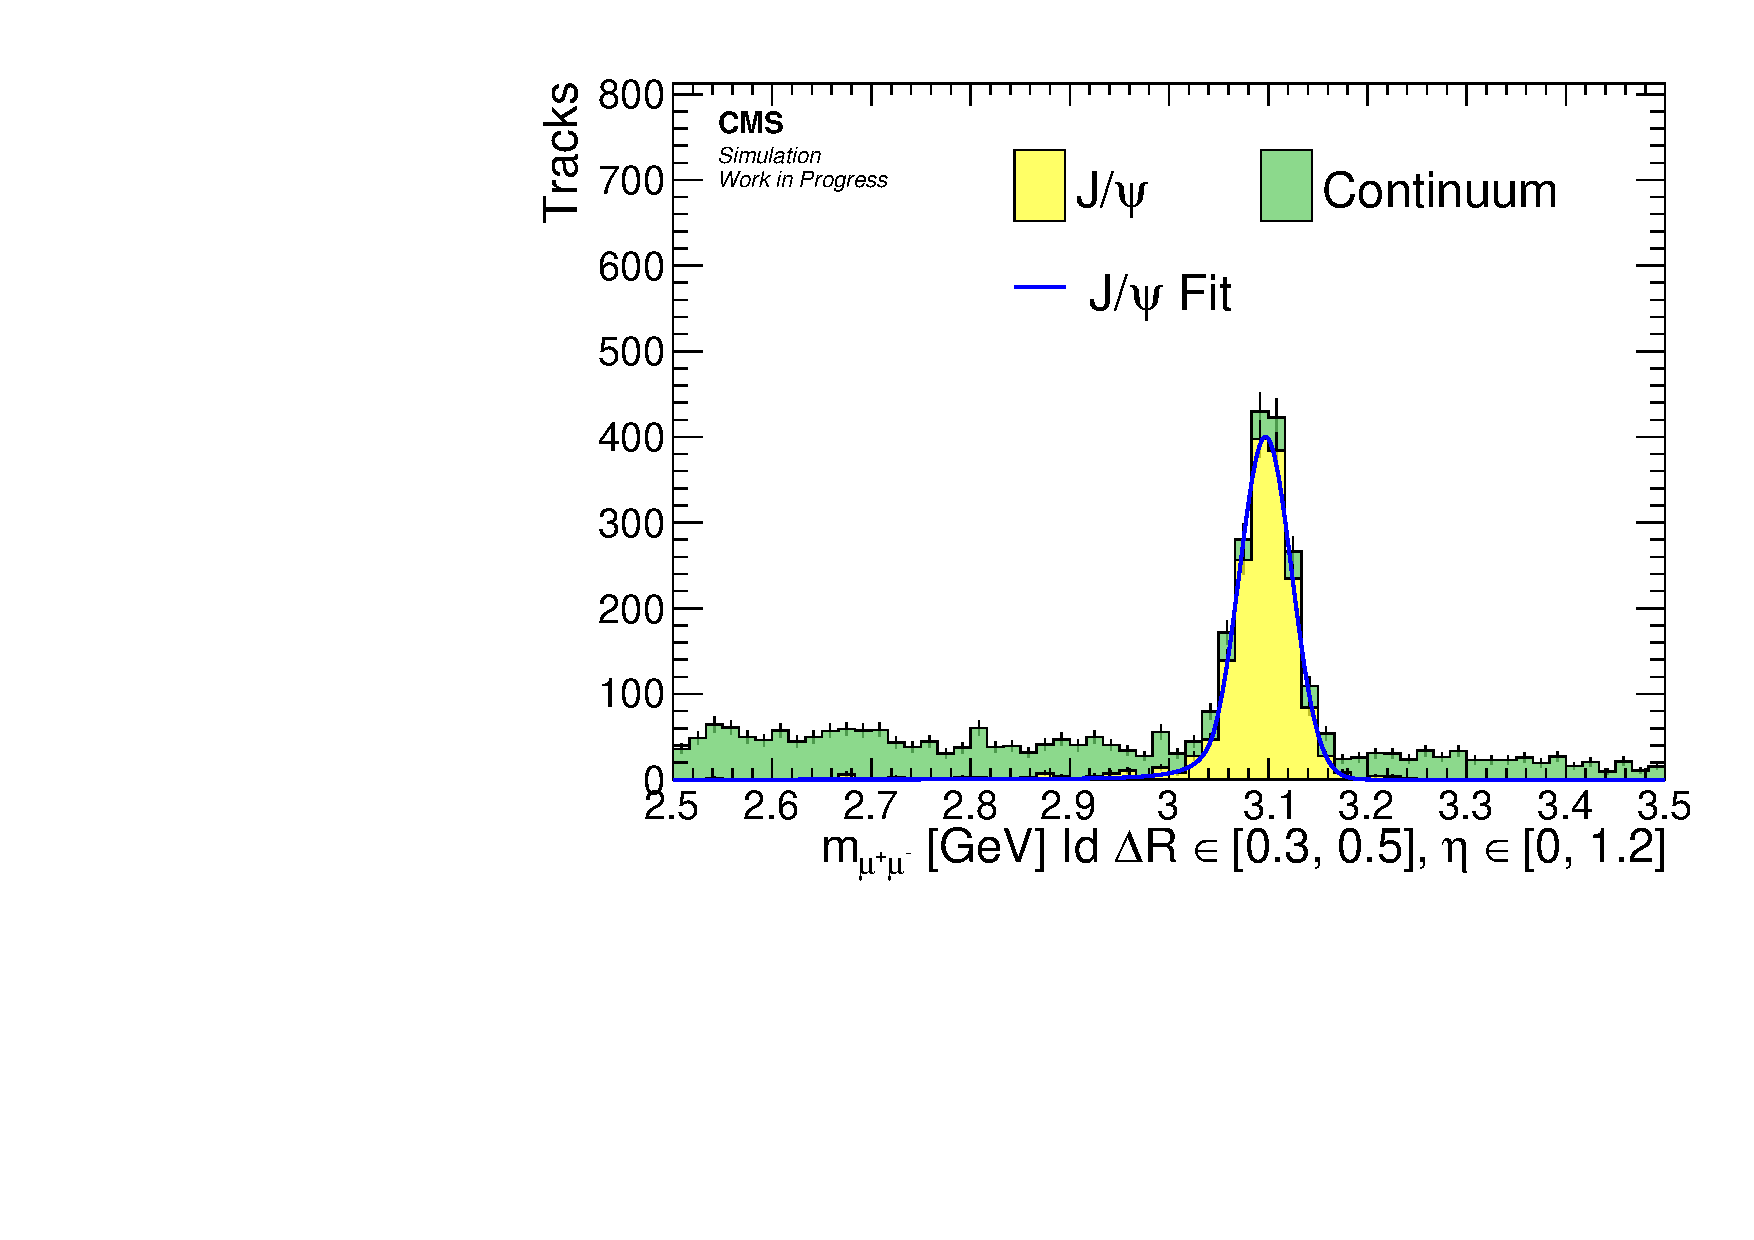
\includegraphics[width=0.32\linewidth]{plots/jpsi_muons_fit_bg_delta_r_single_electron/none_id_invMass_0.3_0.5_0_1.2.pdf}  \,
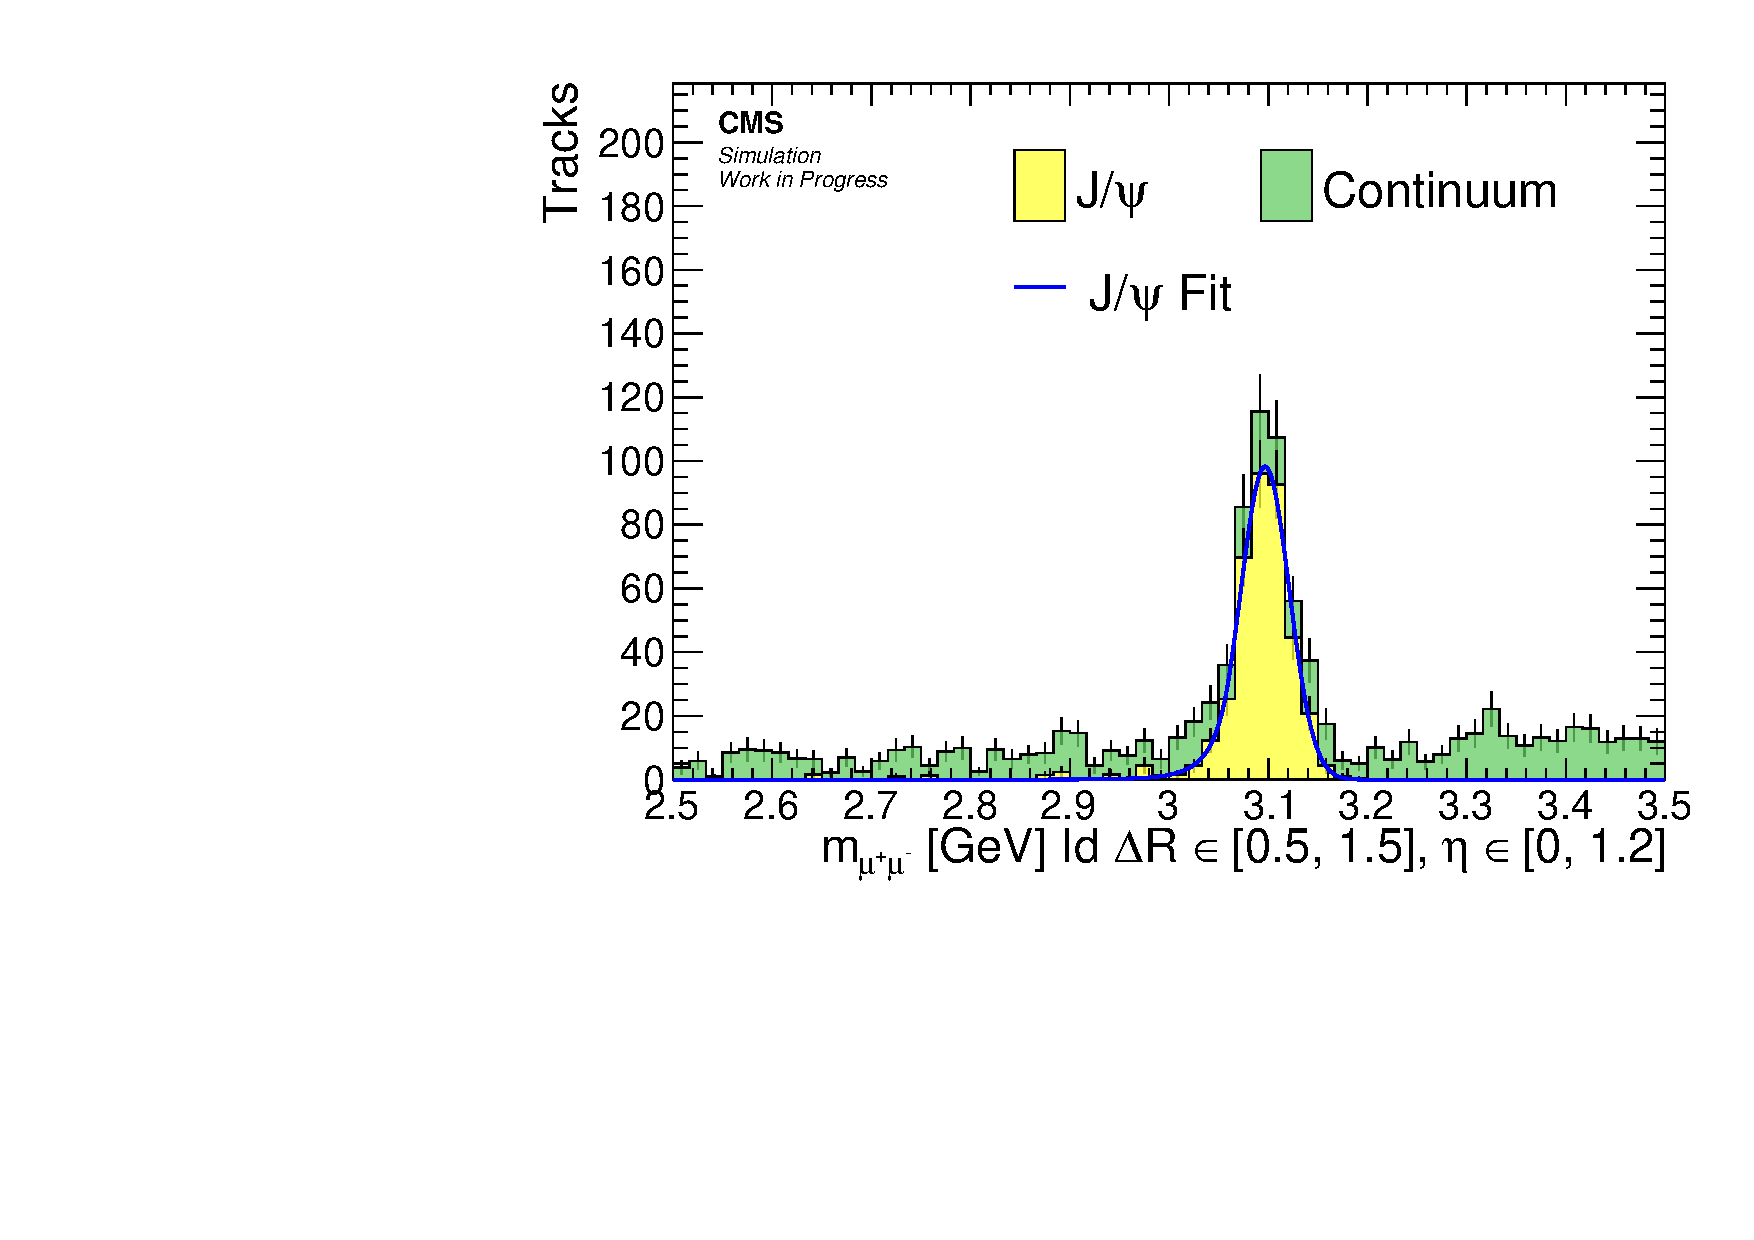
\includegraphics[width=0.32\linewidth]{plots/jpsi_muons_fit_bg_delta_r_single_electron/none_id_invMass_0.5_1.5_0_1.2.pdf} \\
\caption[Simluation barrel muons fits]{Simluation barrel muons fits for denominator (top) and numerator (bottom) for $0<\DR<0.3$  (left), $0.3<\DR<0.5$ (center), $0.5<\DR<1.5$ (right)}
\label{fig:tb-barrel-simulation}
\end{figure}

\begin{figure}[!htbp]
\centering
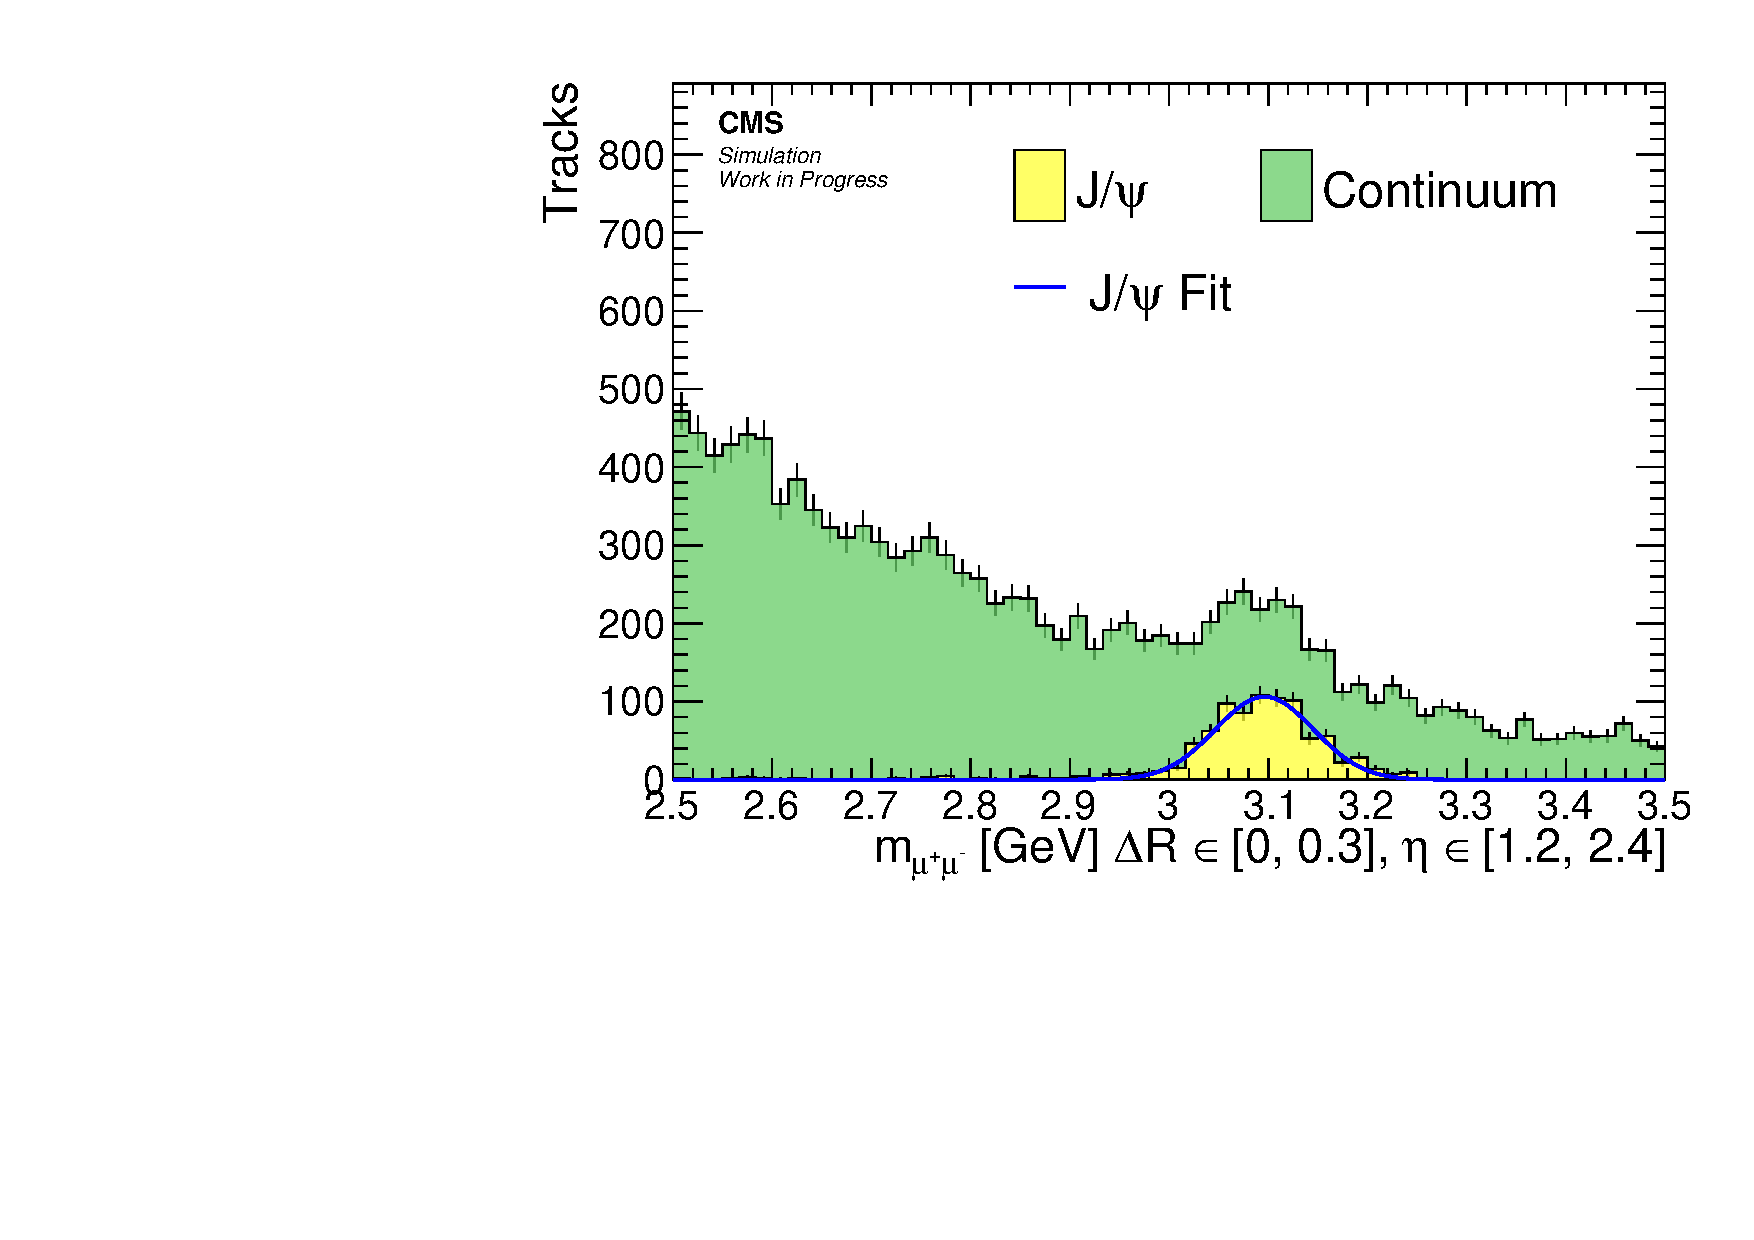
\includegraphics[width=0.32\linewidth]{plots/jpsi_muons_fit_bg_delta_r_single_electron/none_invMass_0_0.3_1.2_2.4.pdf} \,
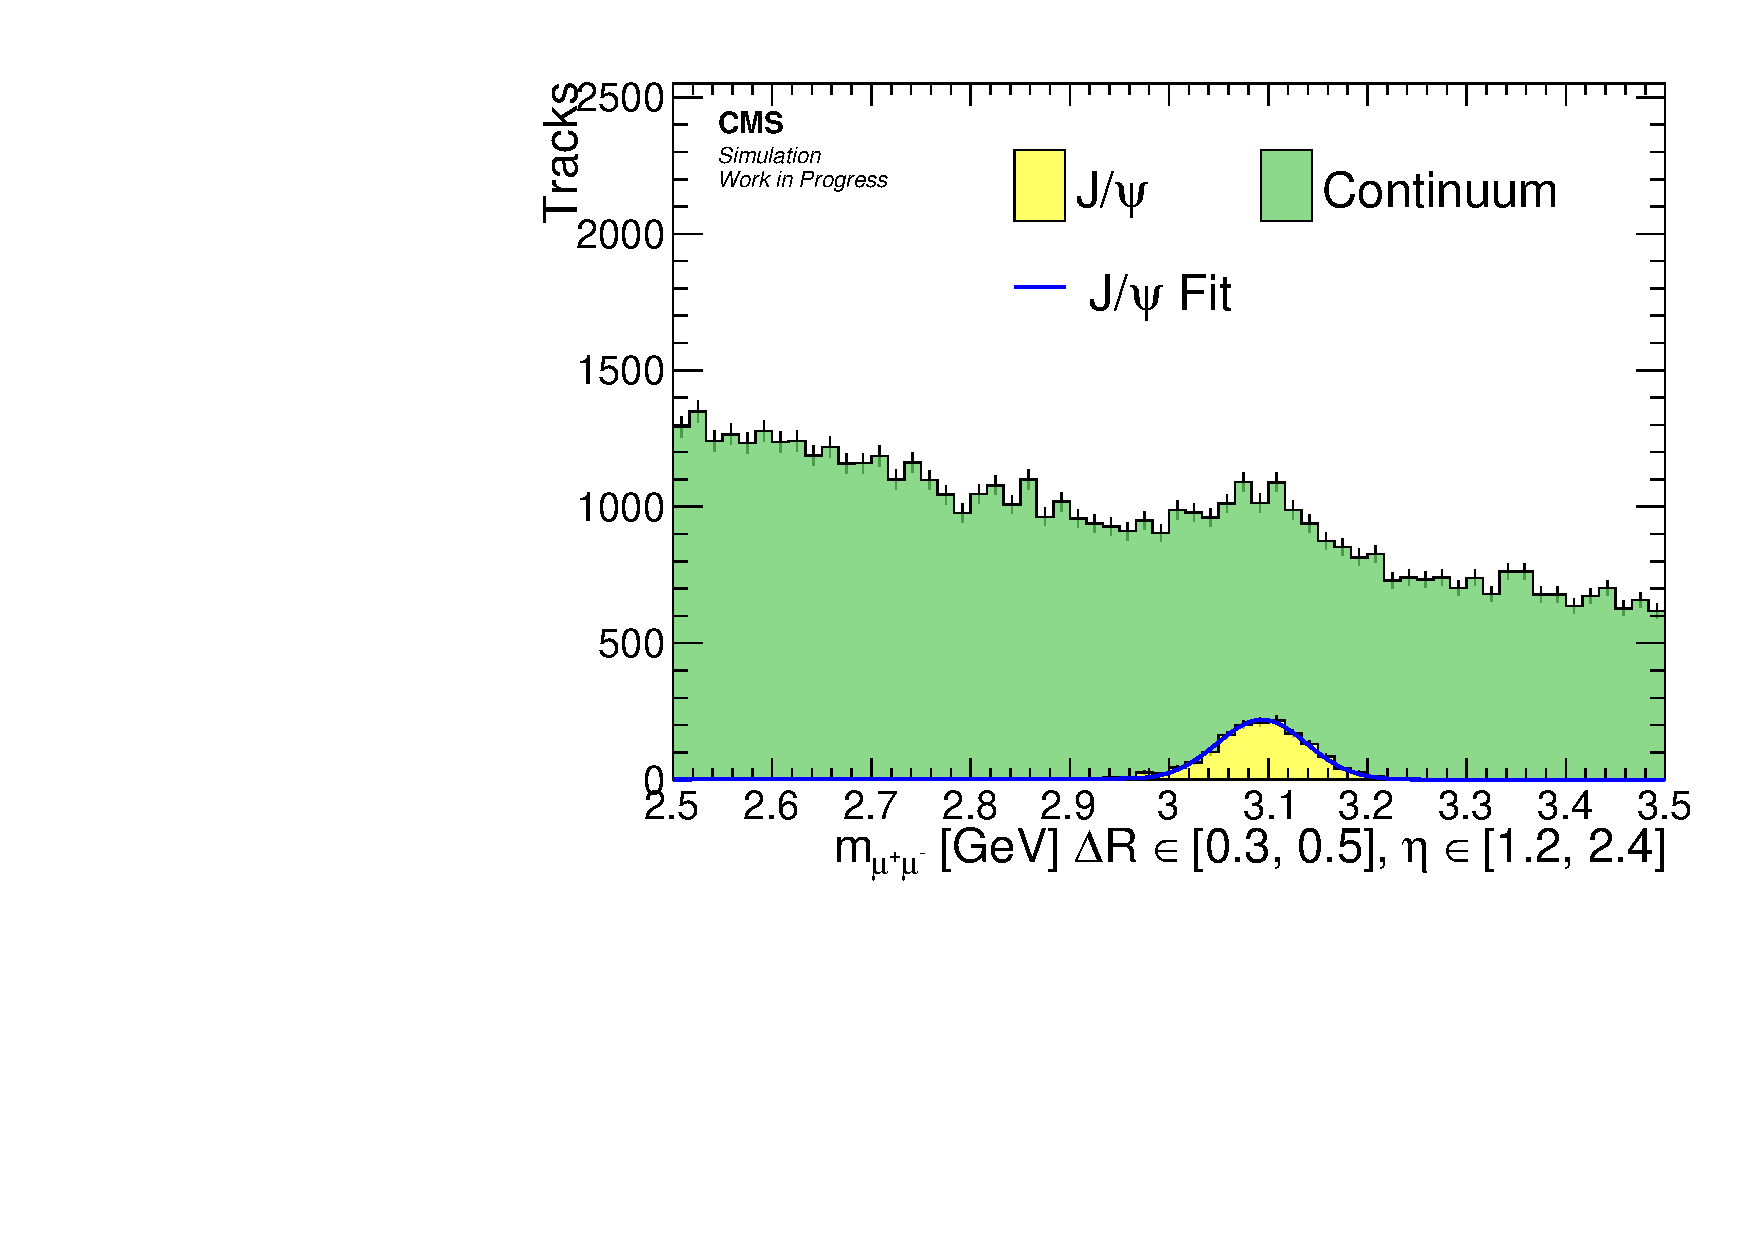
\includegraphics[width=0.32\linewidth]{plots/jpsi_muons_fit_bg_delta_r_single_electron/none_invMass_0.3_0.5_1.2_2.4.pdf} \,
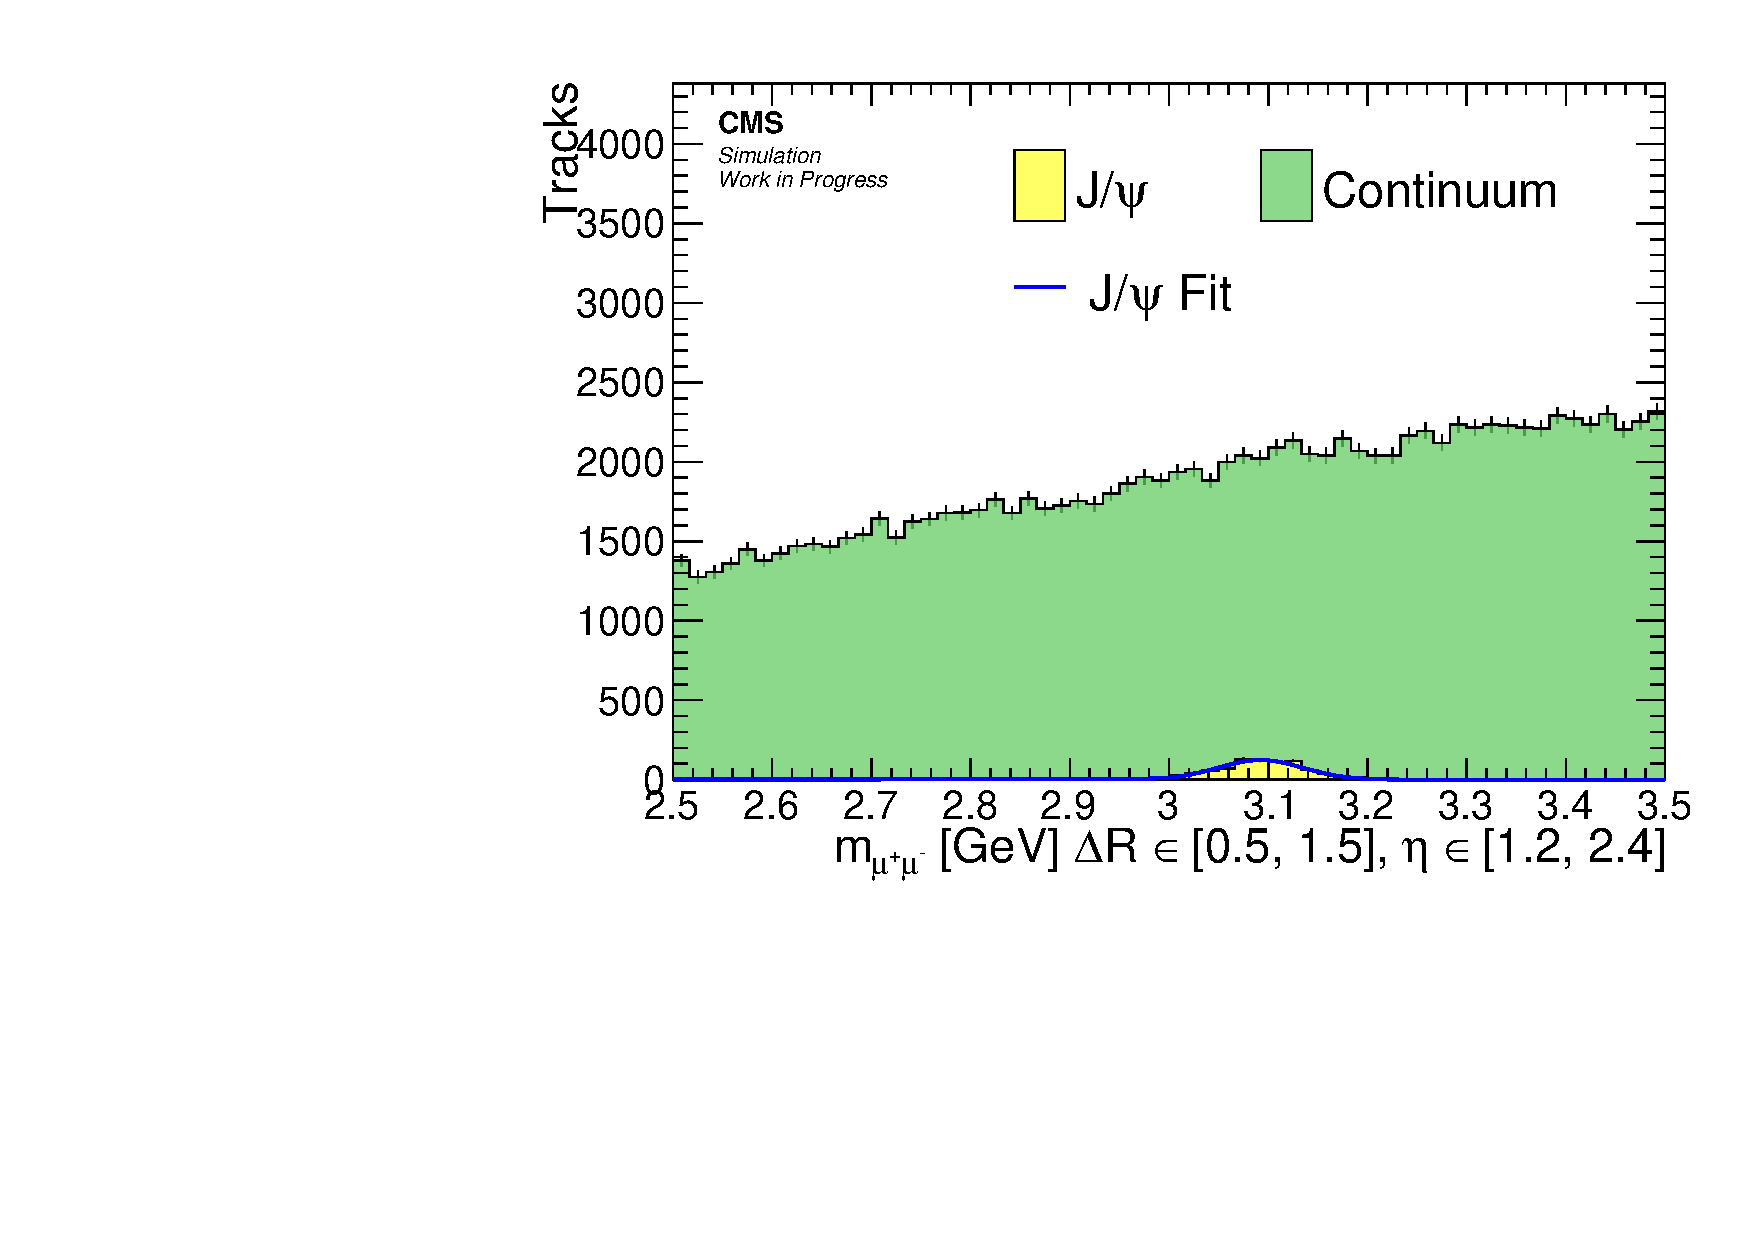
\includegraphics[width=0.32\linewidth]{plots/jpsi_muons_fit_bg_delta_r_single_electron/none_invMass_0.5_1.5_1.2_2.4.pdf} \\
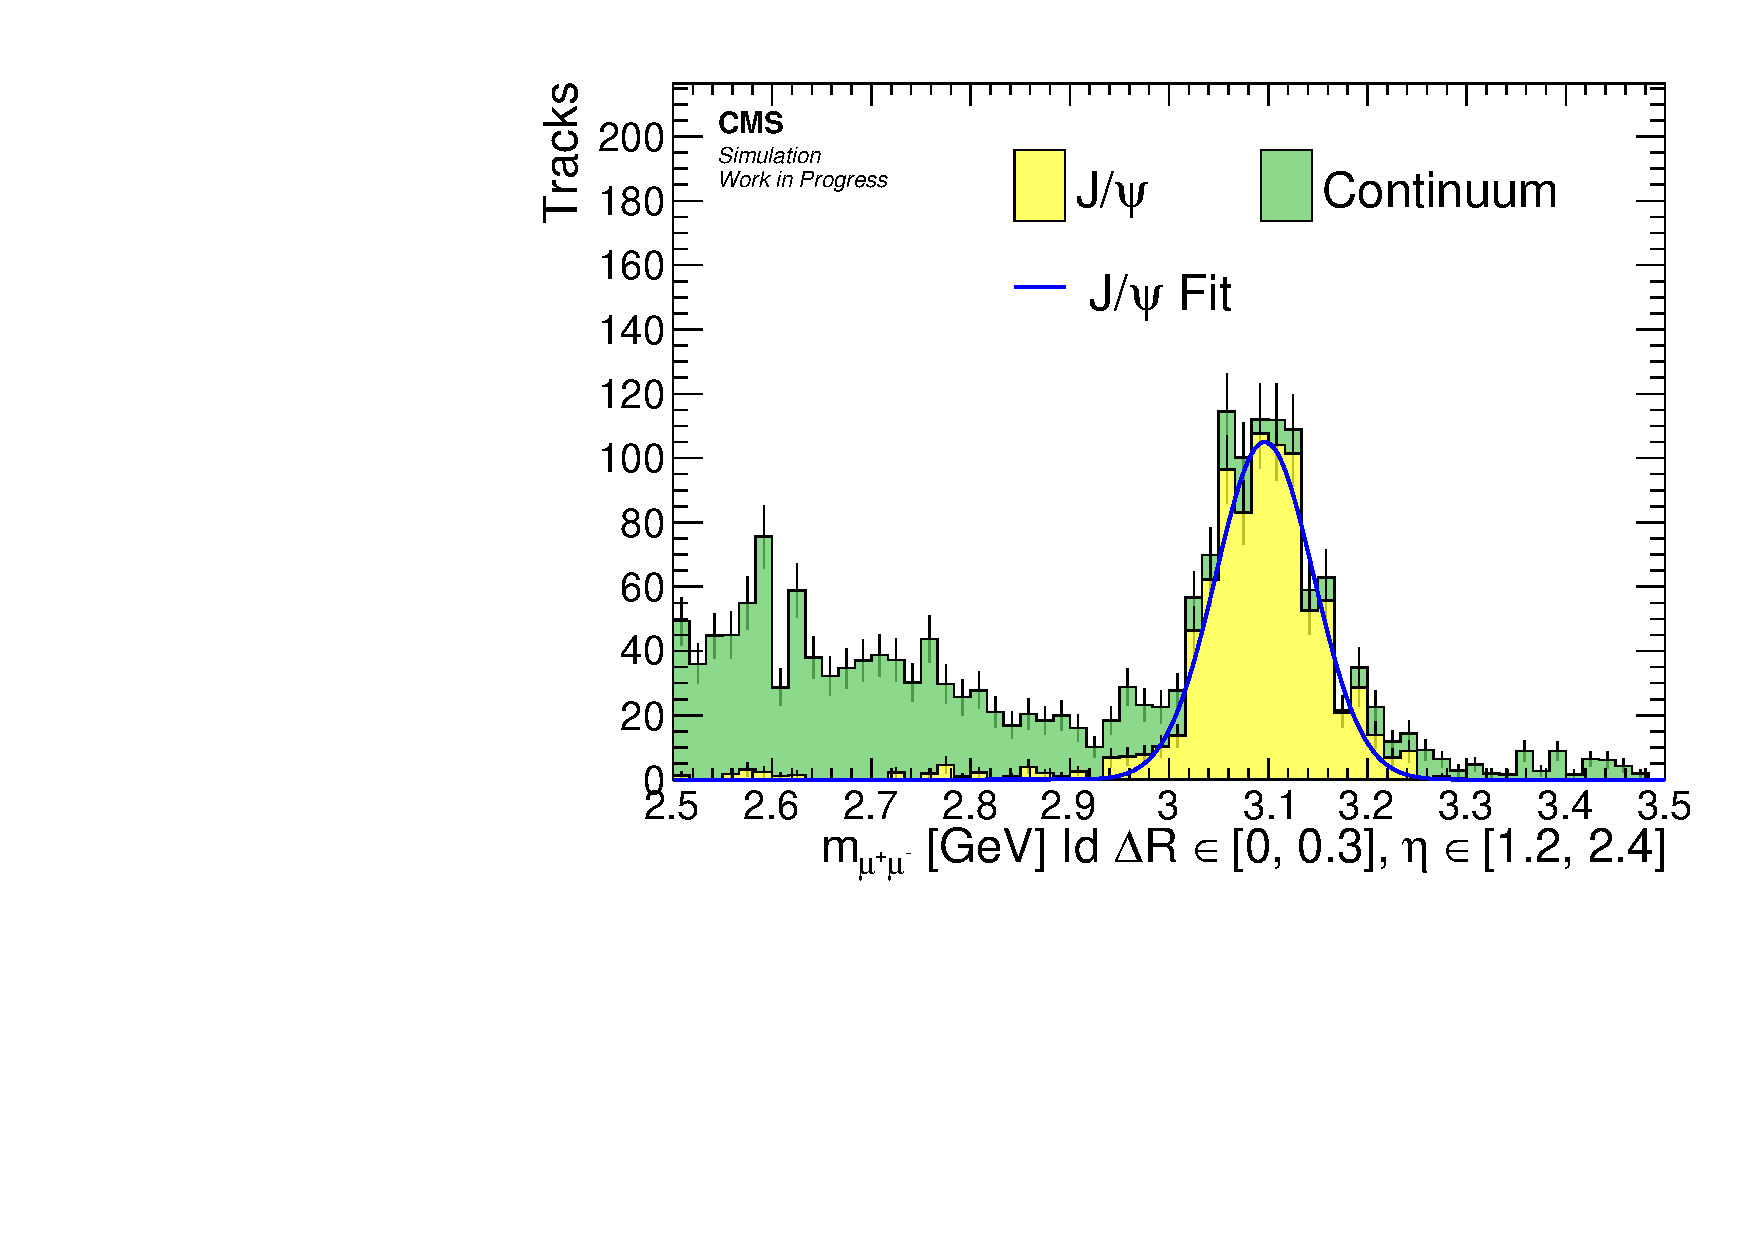
\includegraphics[width=0.32\linewidth]{plots/jpsi_muons_fit_bg_delta_r_single_electron/none_id_invMass_0_0.3_1.2_2.4.pdf} \,
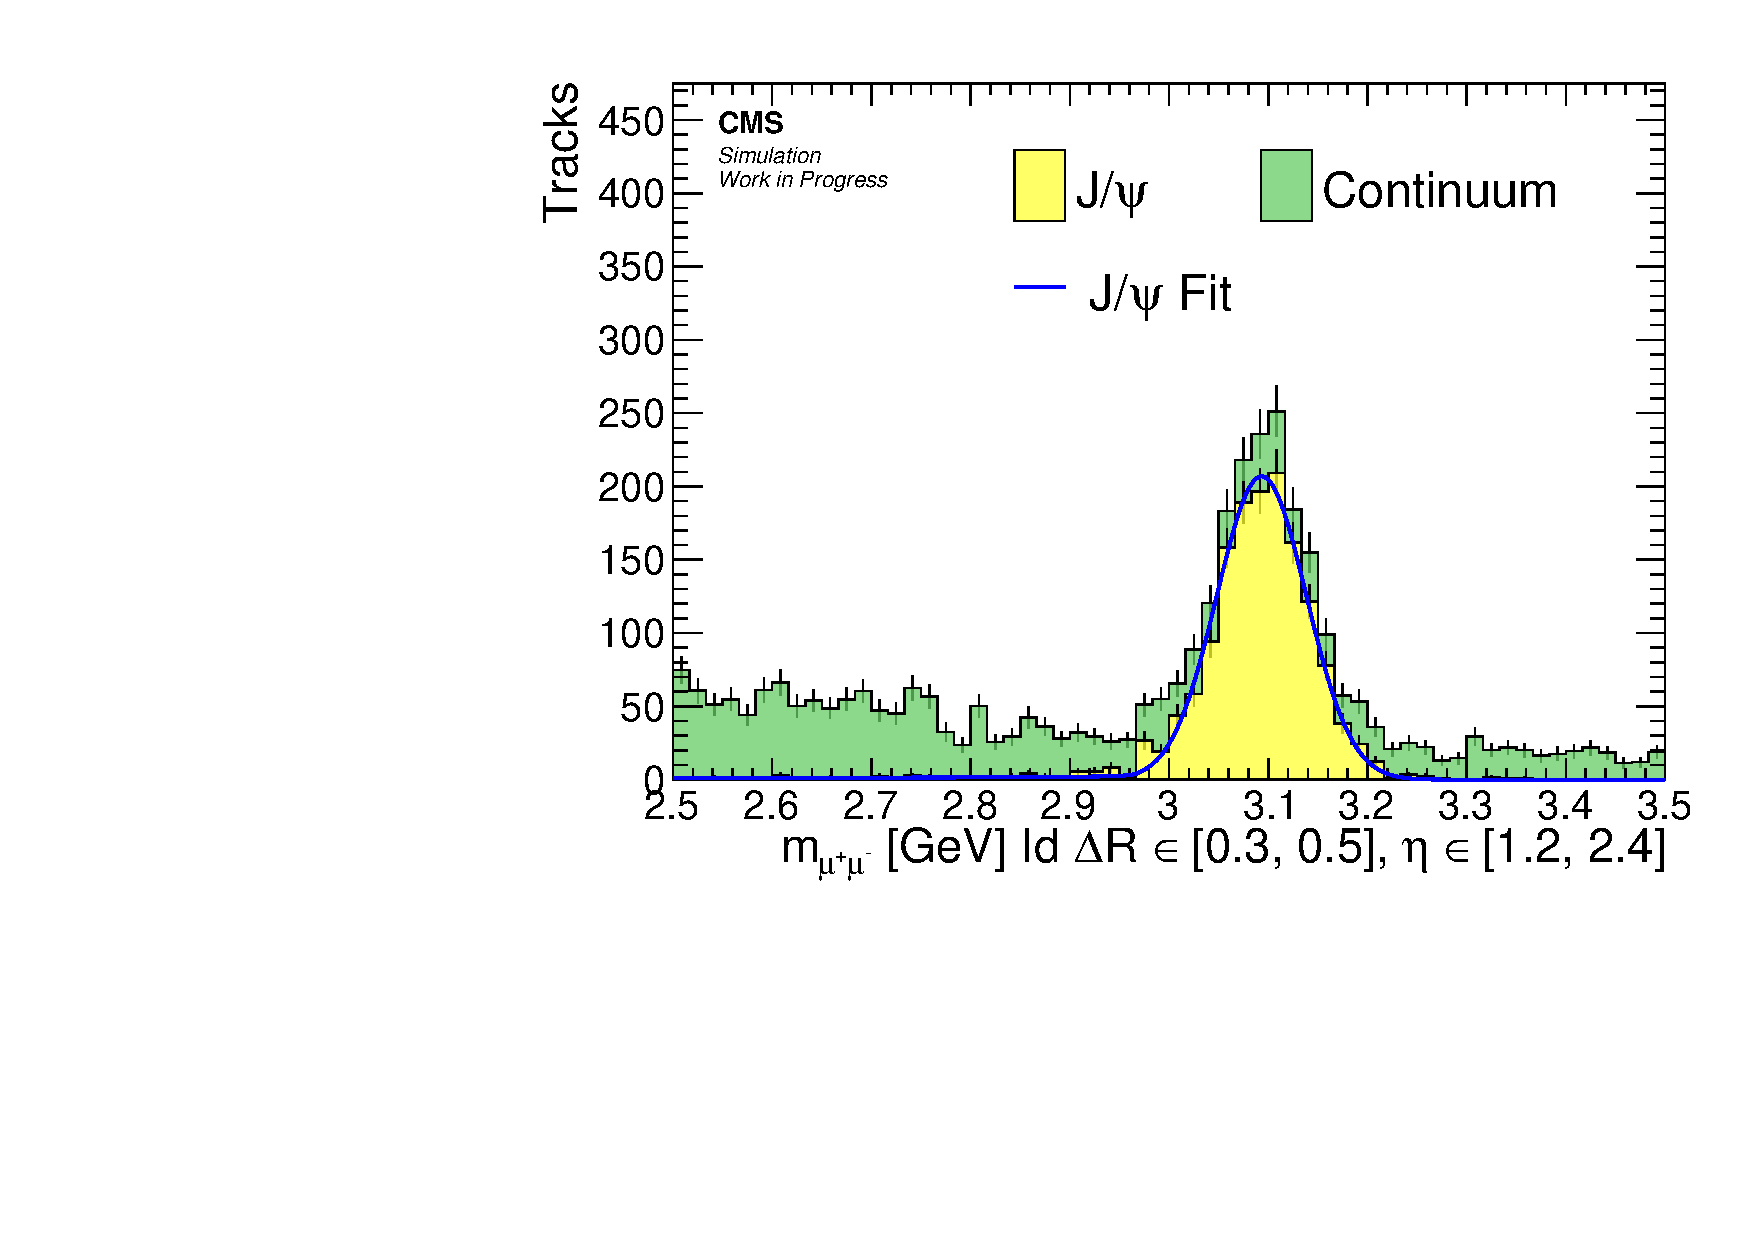
\includegraphics[width=0.32\linewidth]{plots/jpsi_muons_fit_bg_delta_r_single_electron/none_id_invMass_0.3_0.5_1.2_2.4.pdf} \,
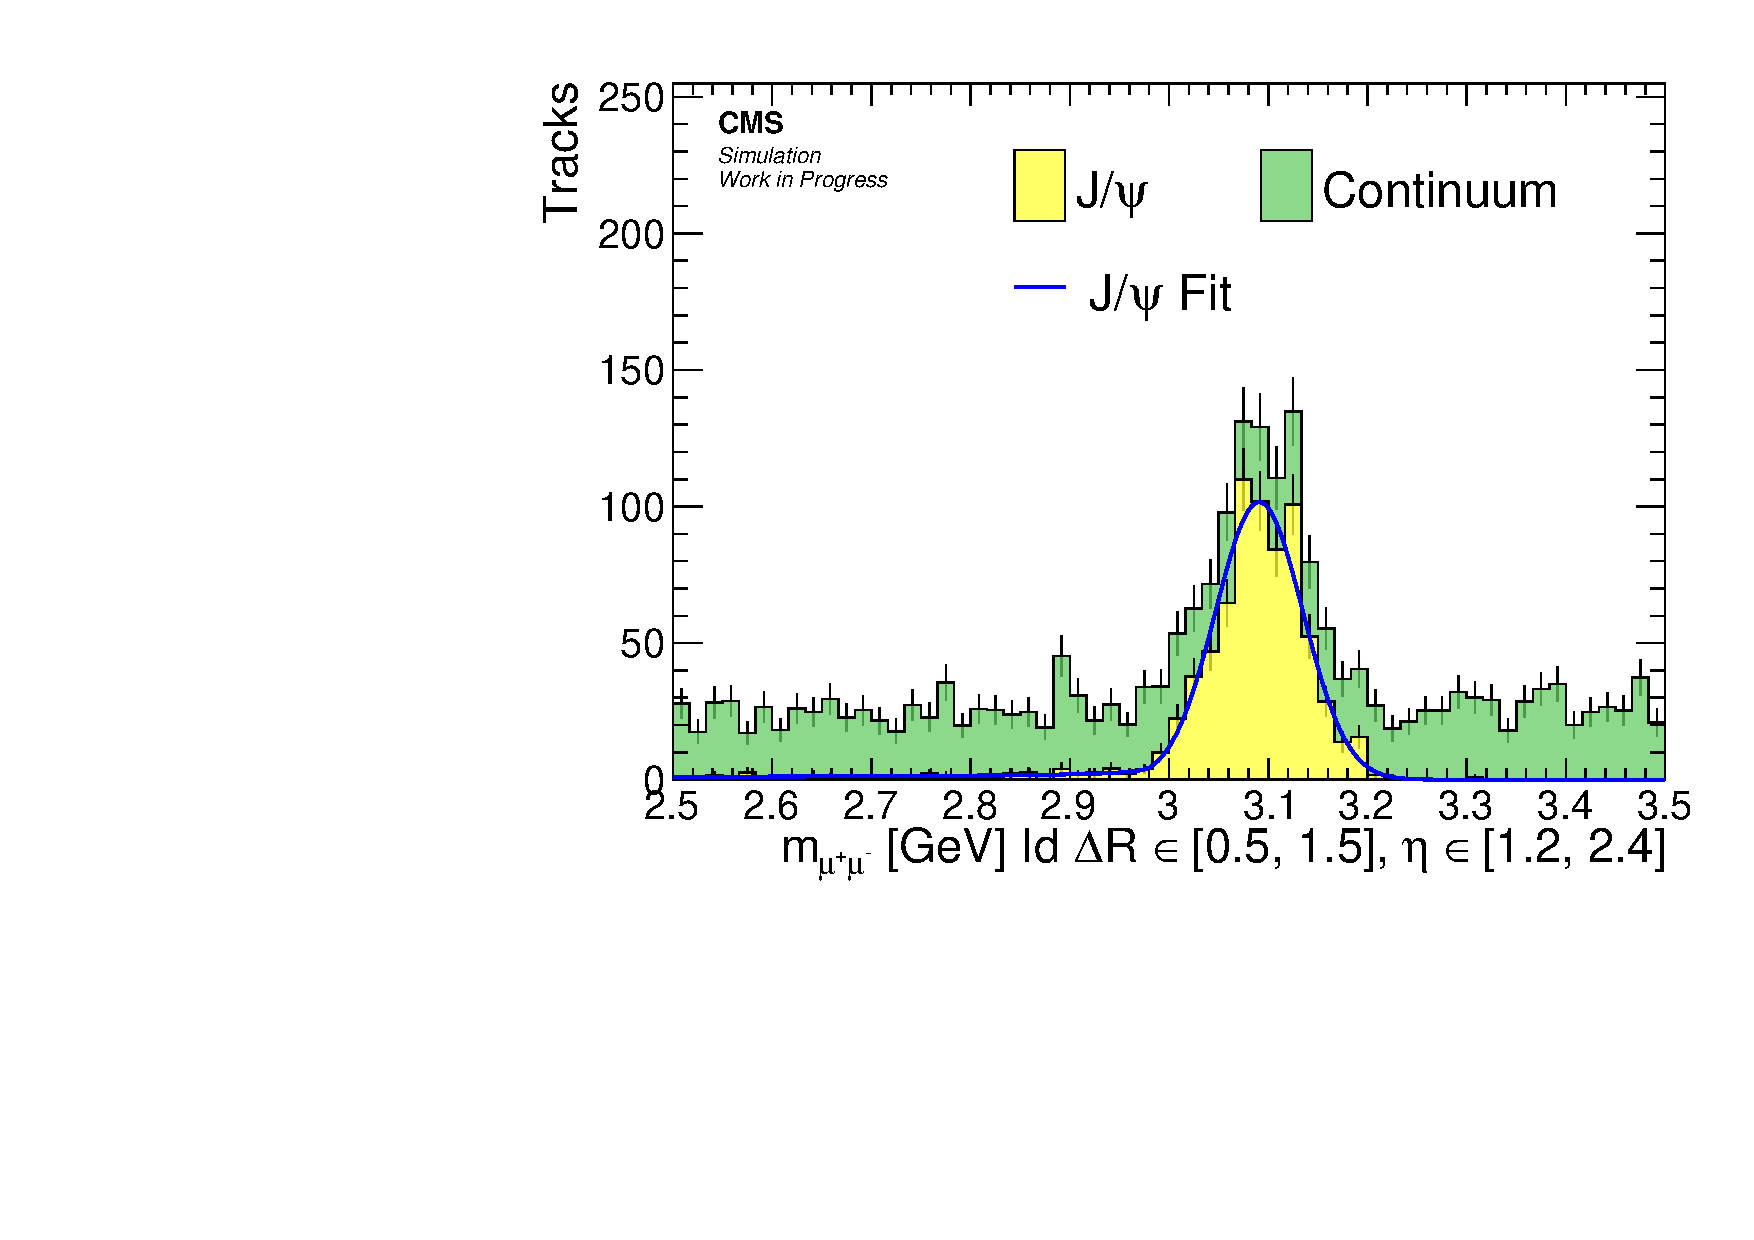
\includegraphics[width=0.32\linewidth]{plots/jpsi_muons_fit_bg_delta_r_single_electron/none_id_invMass_0.5_1.5_1.2_2.4.pdf}  \\
\caption[Simluation endcaps muons fits]{Simluation endcaps muons fits for denominator (top) and numerator (bottom) for $0<\DR<0.3$  (left), $0.3<\DR<0.5$ (center), $0.5<\DR<1.5$ (right)}
\label{fig:tb-endcaps-simulation}
\end{figure}

\begin{figure}[!htbp]
\centering
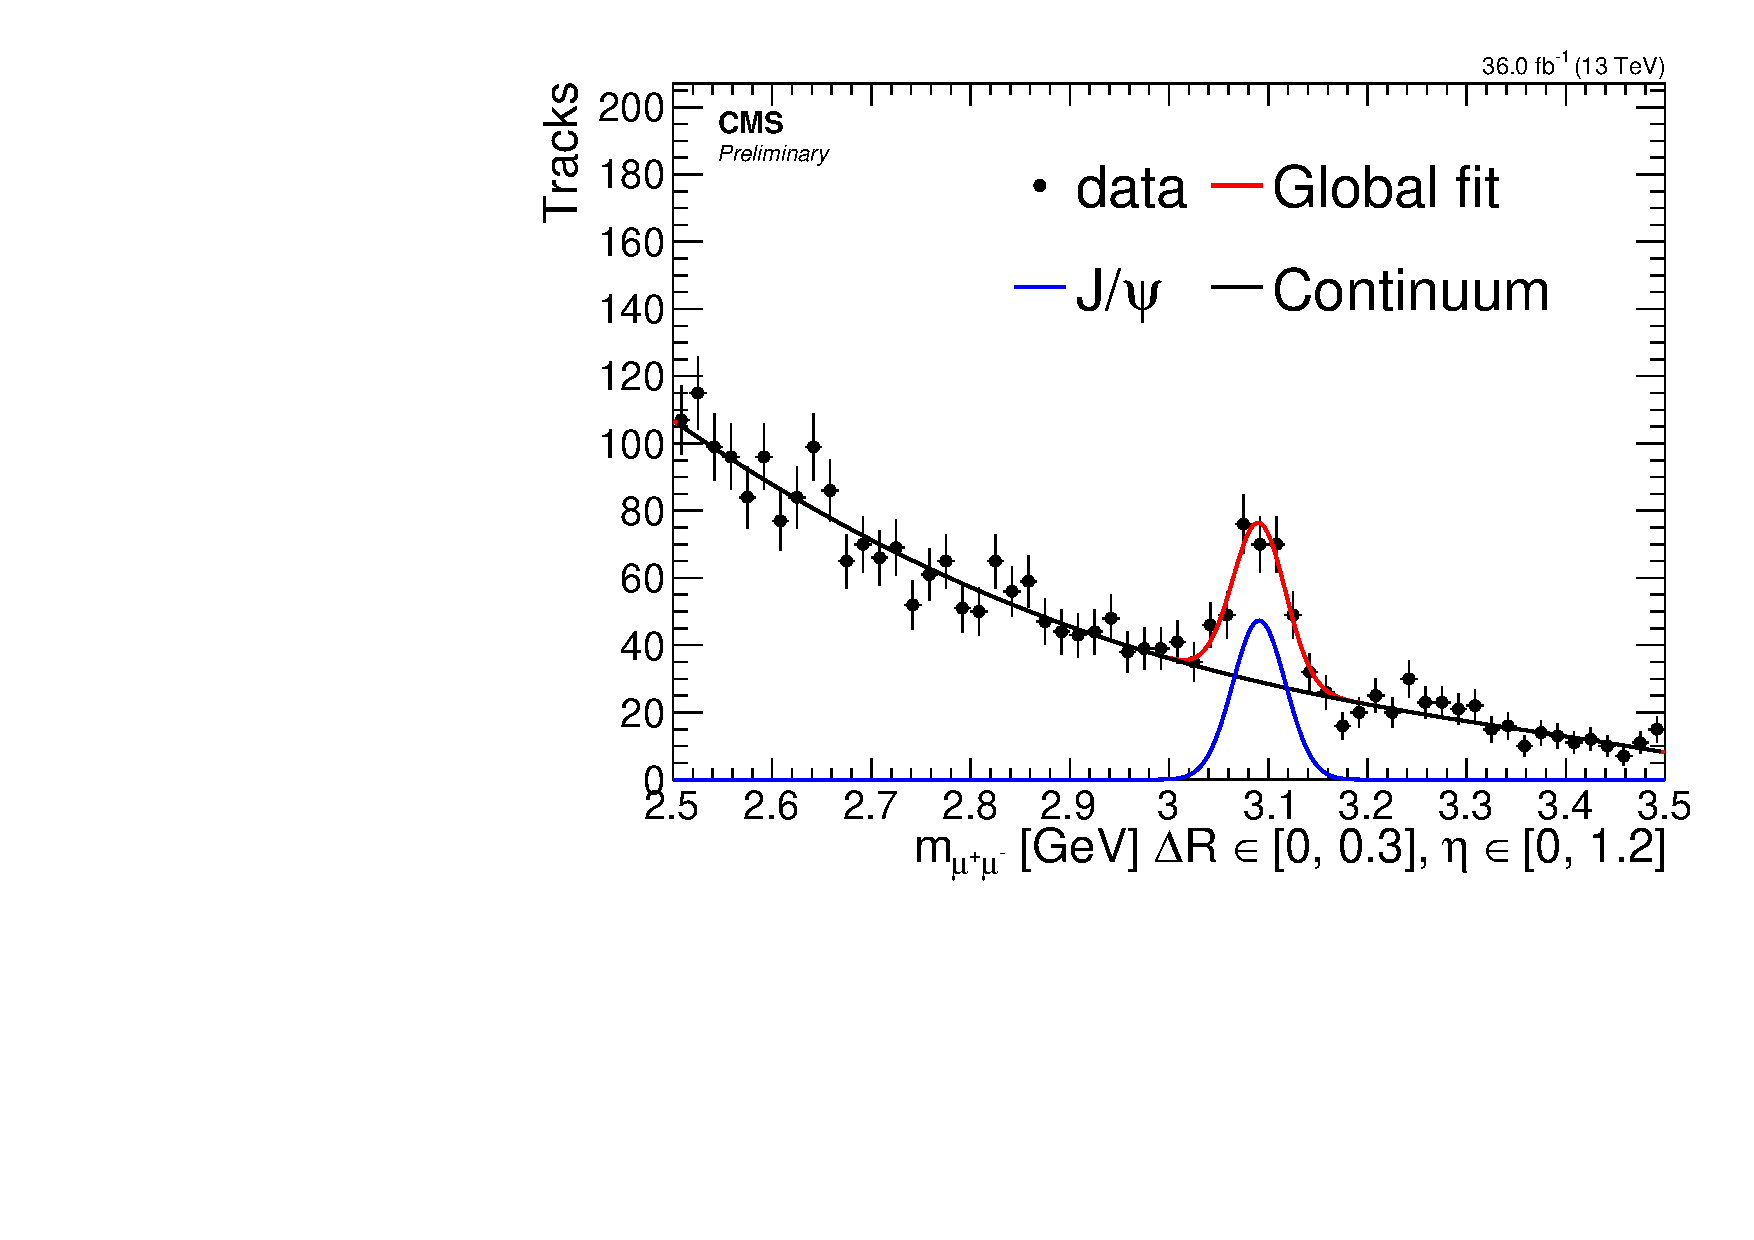
\includegraphics[width=0.32\linewidth]{plots/jpsi_muons_fit_data_delta_r_single_electron/none_invMass_0_0.3_0_1.2.pdf} \,
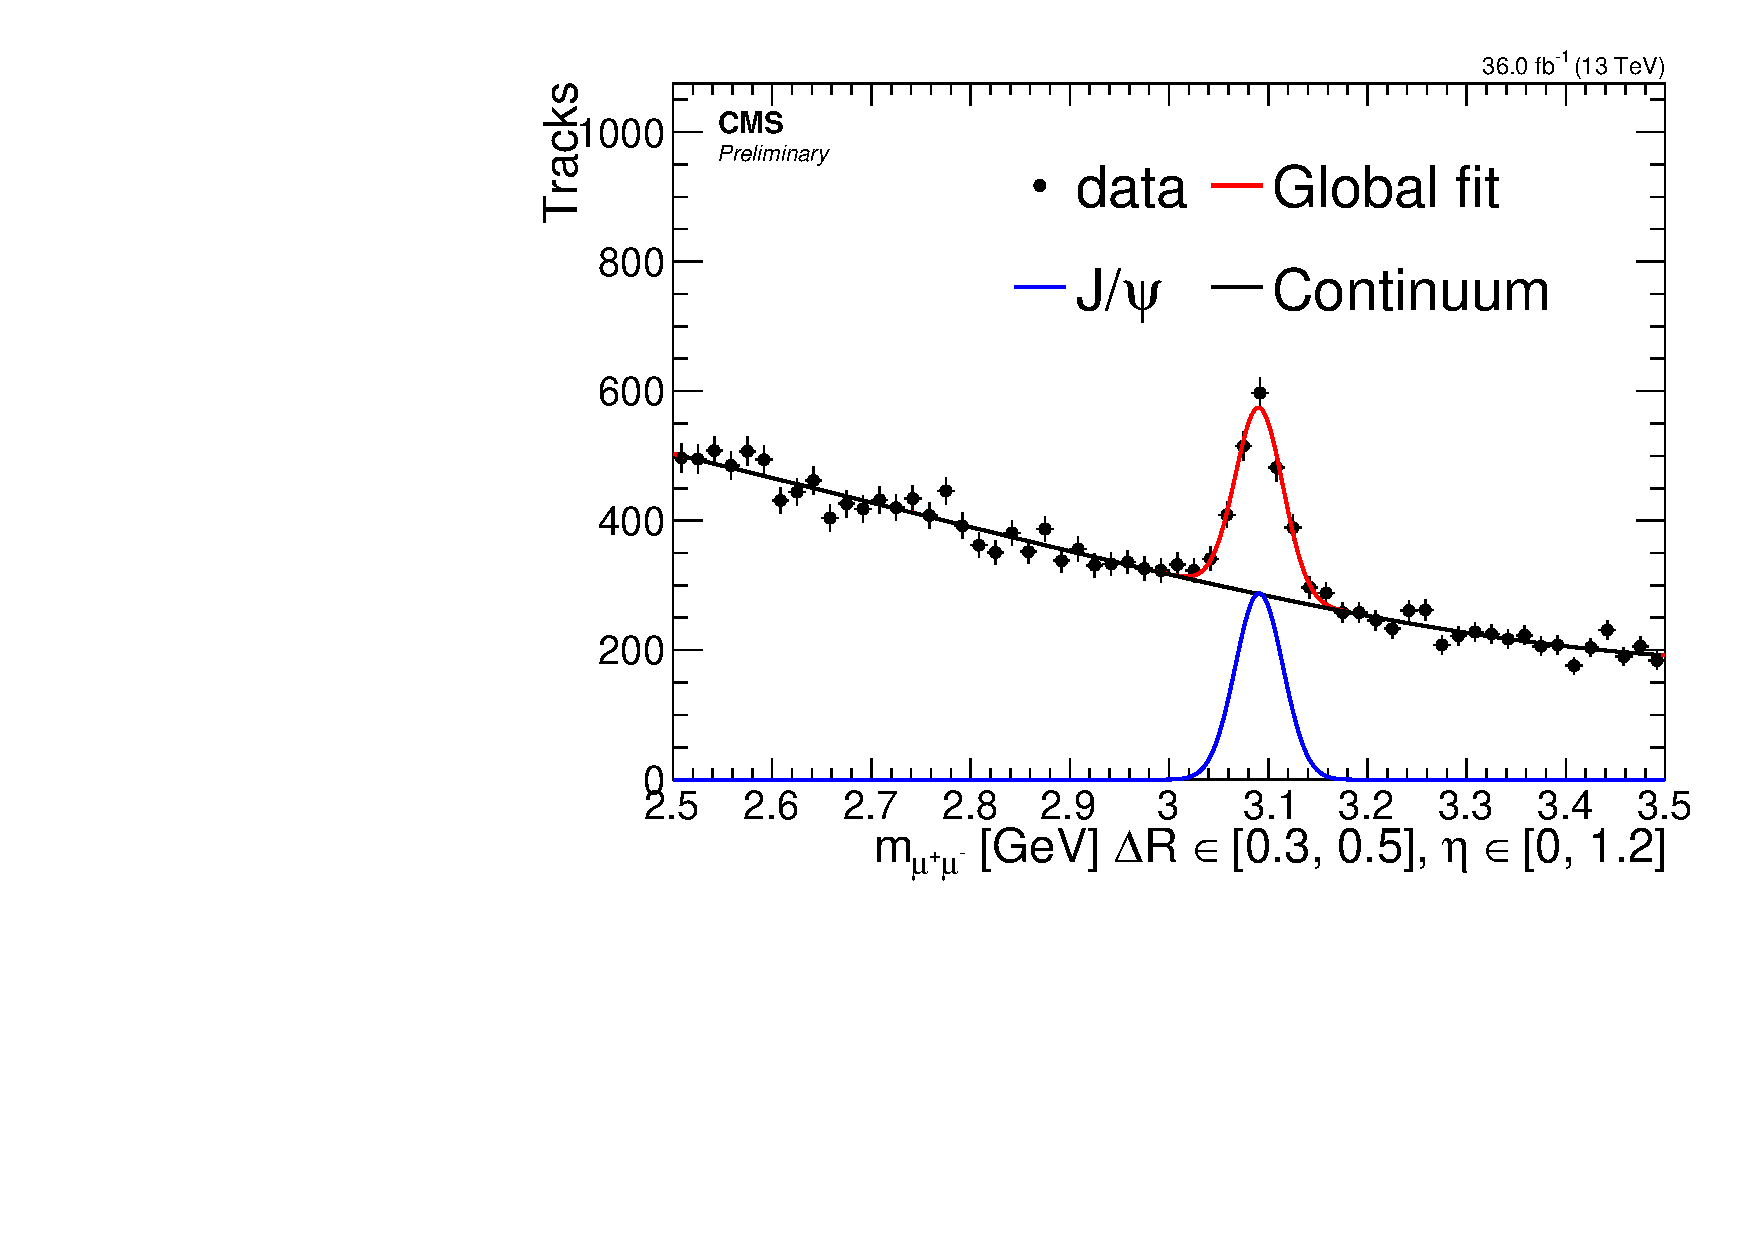
\includegraphics[width=0.32\linewidth]{plots/jpsi_muons_fit_data_delta_r_single_electron/none_invMass_0.3_0.5_0_1.2.pdf}  \,
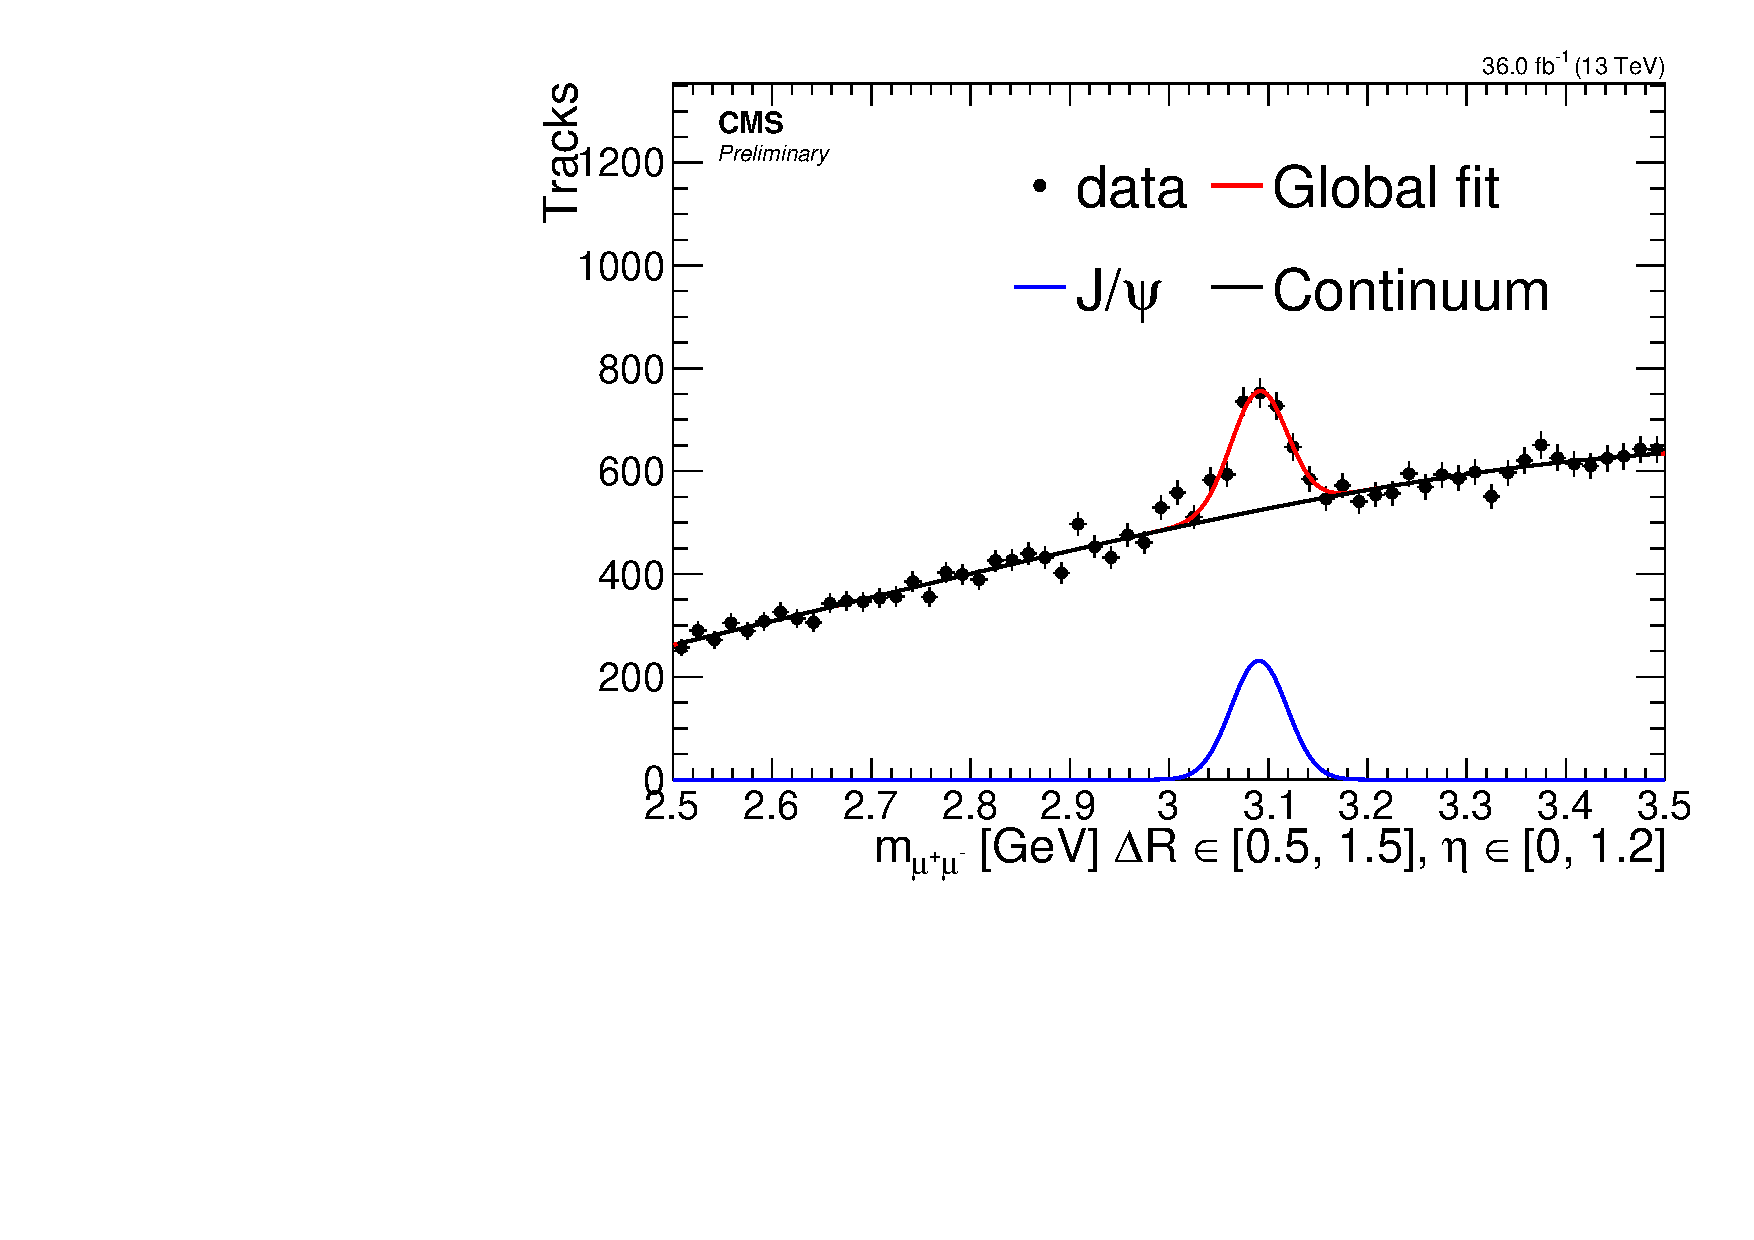
\includegraphics[width=0.32\linewidth]{plots/jpsi_muons_fit_data_delta_r_single_electron/none_invMass_0.5_1.5_0_1.2.pdf} \\
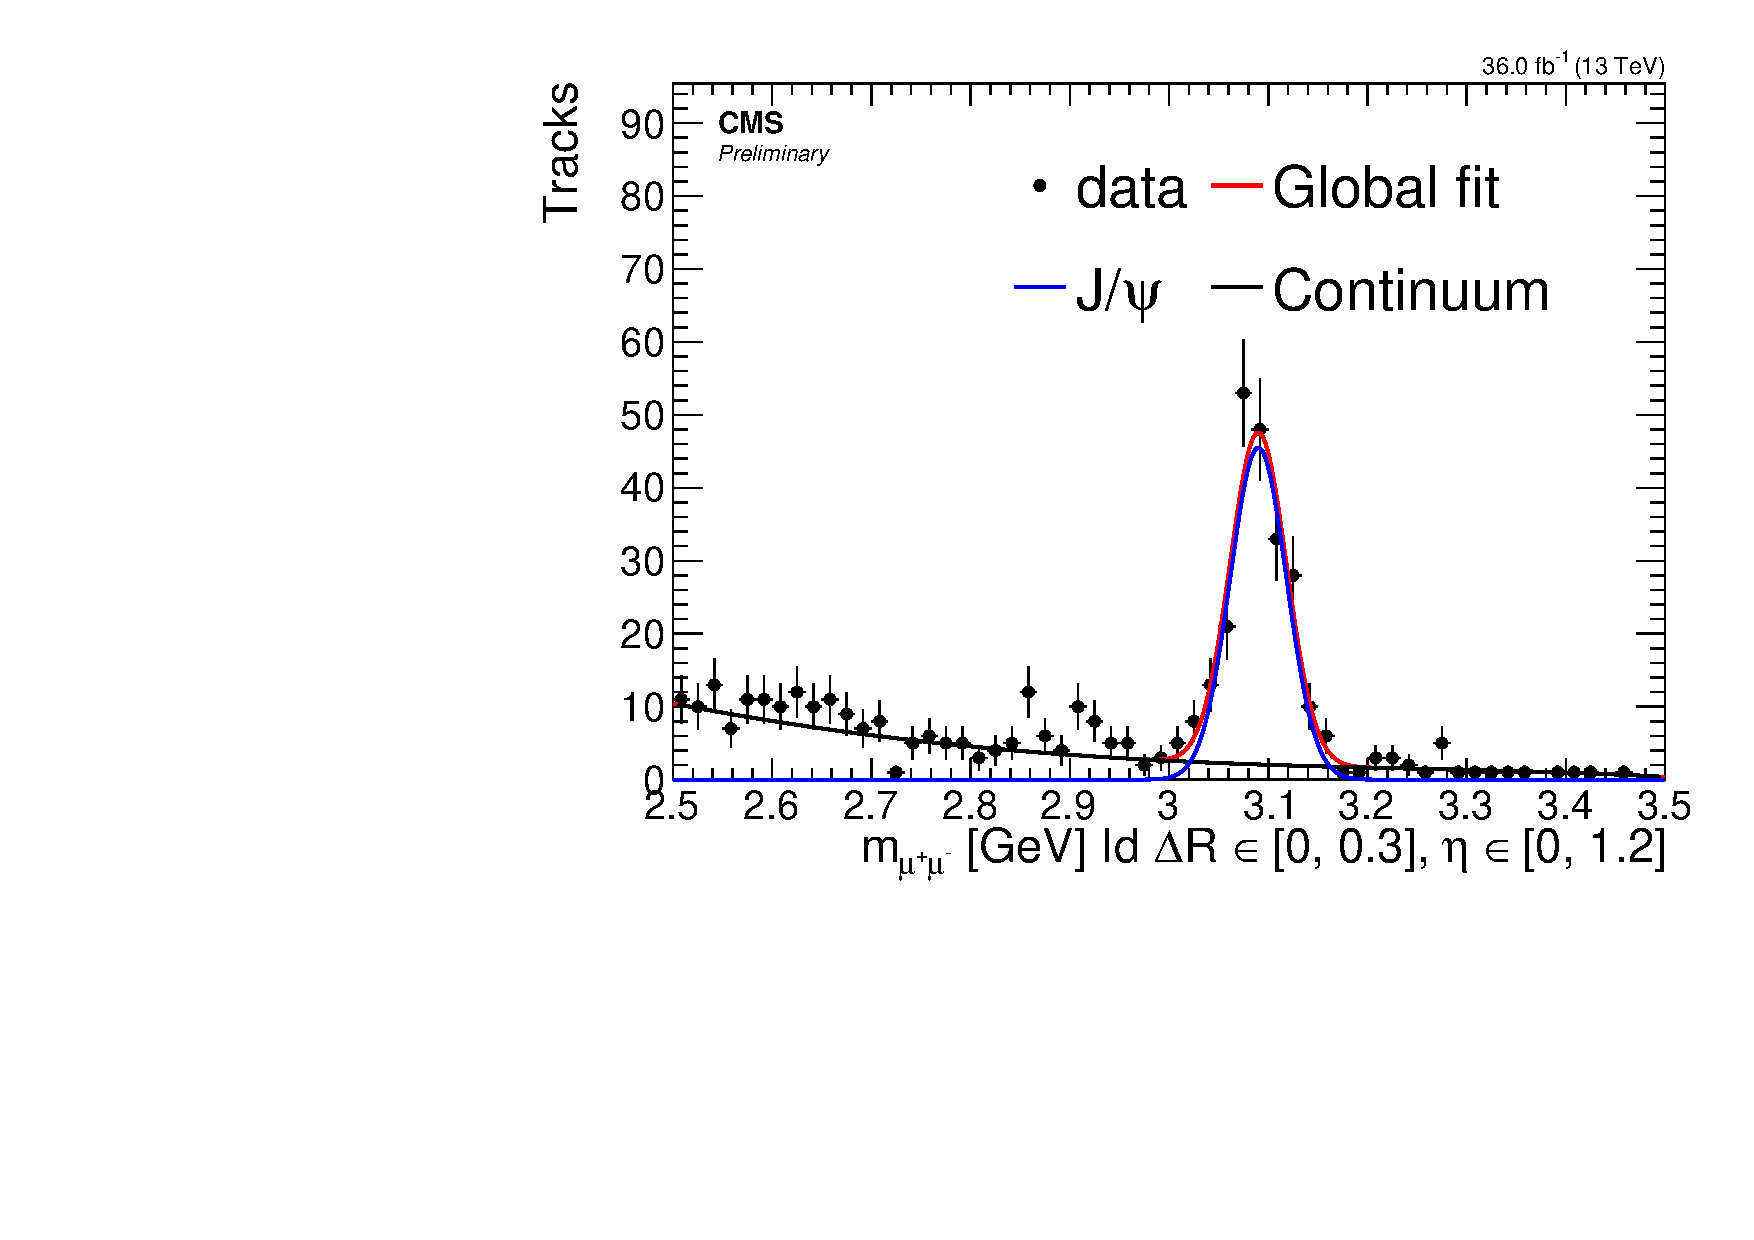
\includegraphics[width=0.32\linewidth]{plots/jpsi_muons_fit_data_delta_r_single_electron/none_id_invMass_0_0.3_0_1.2.pdf} \,
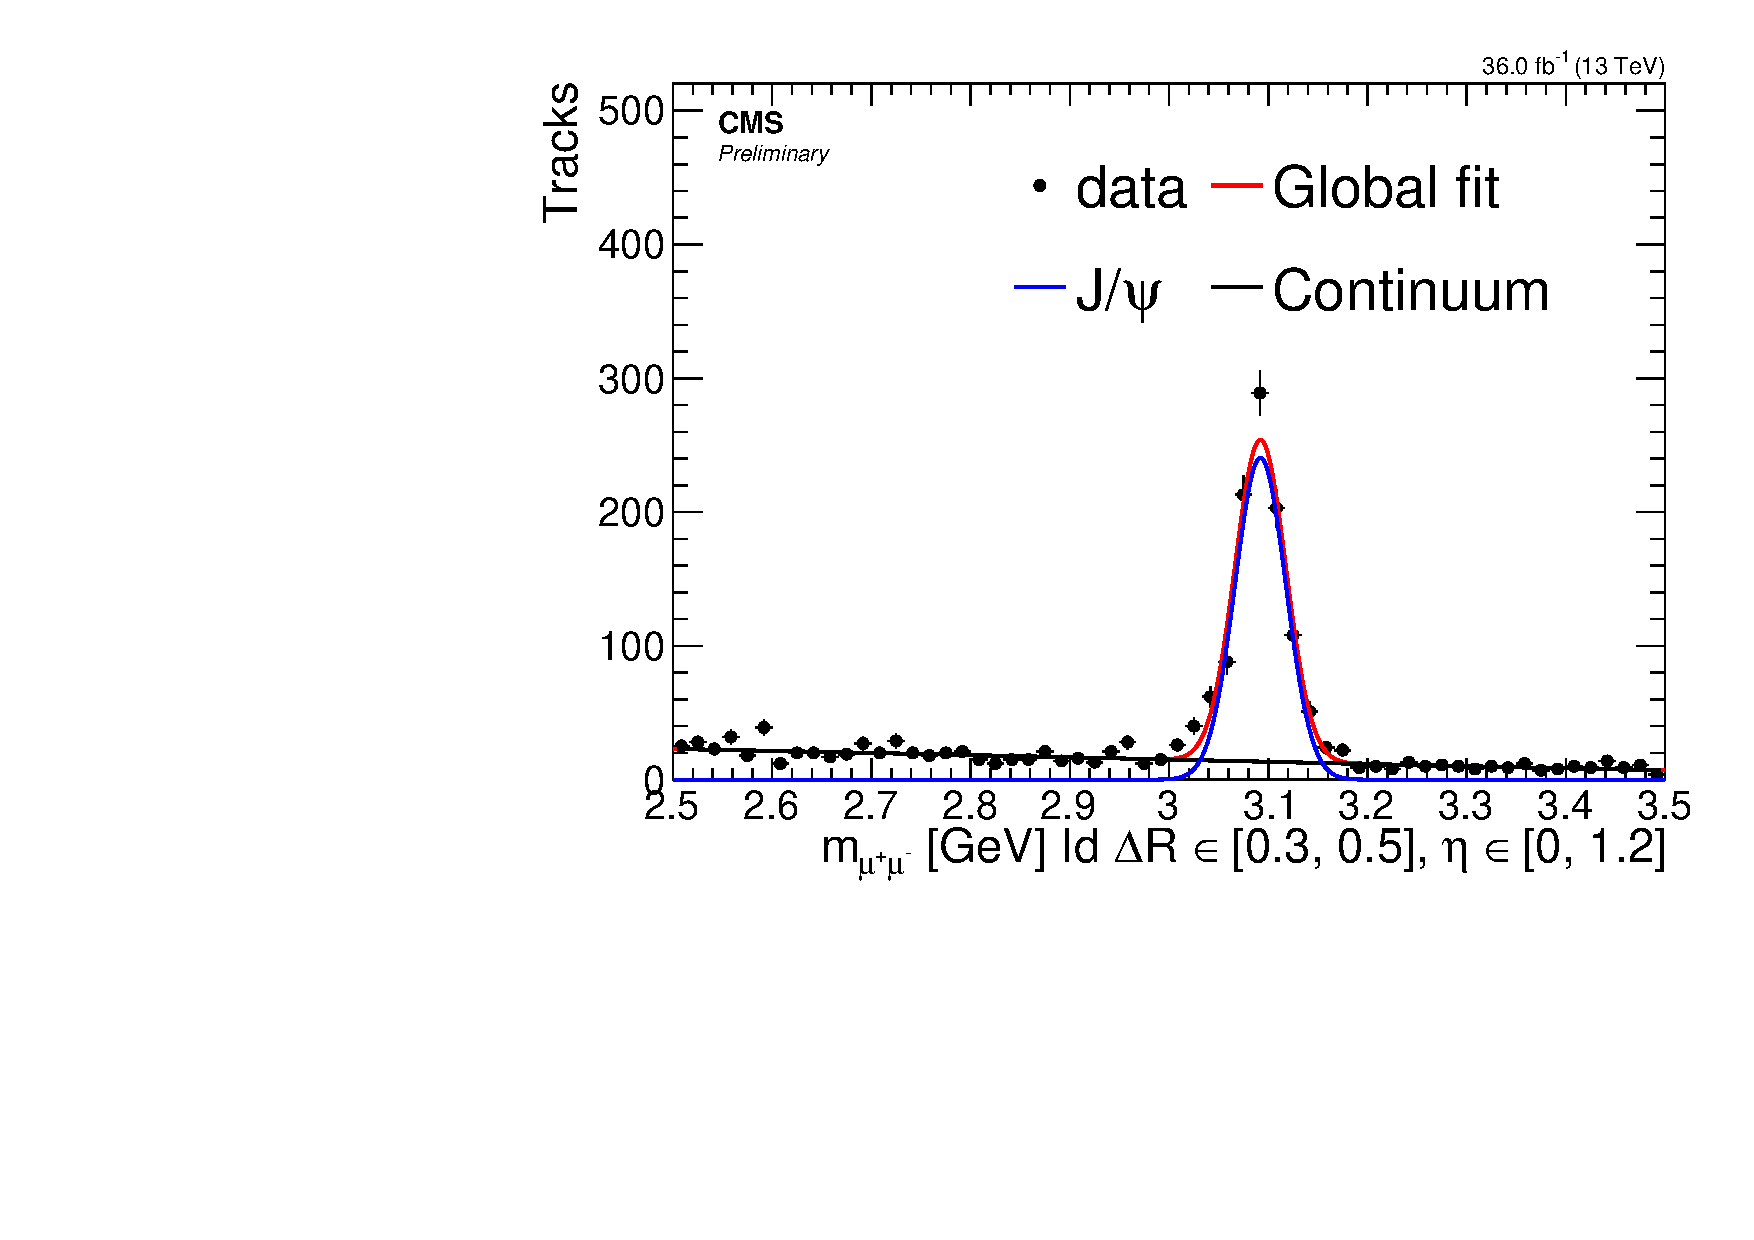
\includegraphics[width=0.32\linewidth]{plots/jpsi_muons_fit_data_delta_r_single_electron/none_id_invMass_0.3_0.5_0_1.2.pdf}  \,
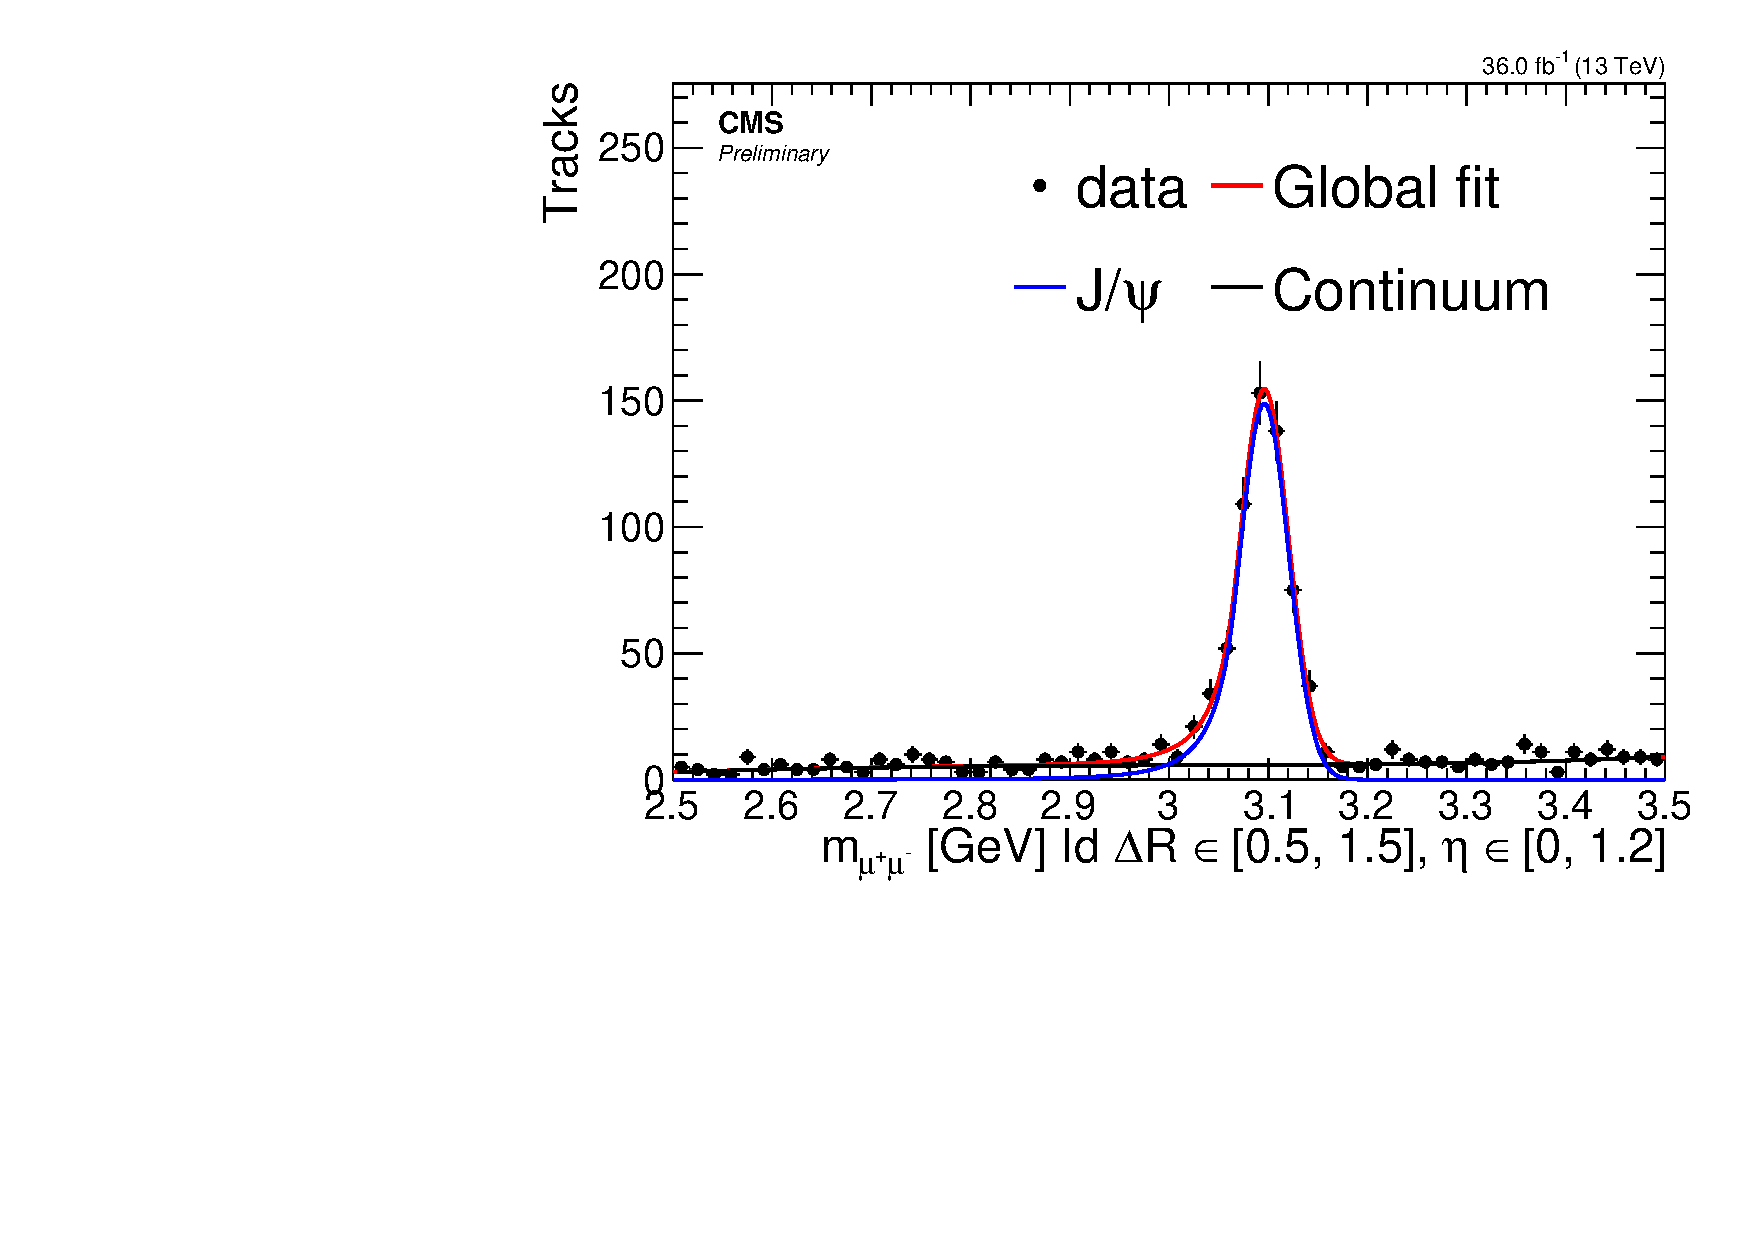
\includegraphics[width=0.32\linewidth]{plots/jpsi_muons_fit_data_delta_r_single_electron/none_id_invMass_0.5_1.5_0_1.2.pdf} \\
\caption[Data barrel muons fits]{Data barrel muons fits for denominator (top) and numerator (bottom) for $0<\DR<0.3$  (left), $0.3<\DR<0.5$ (center), $0.5<\DR<1.5$ (right)}
\label{fig:tb-barrel-data}
\end{figure}

\begin{figure}[!htbp]
\centering
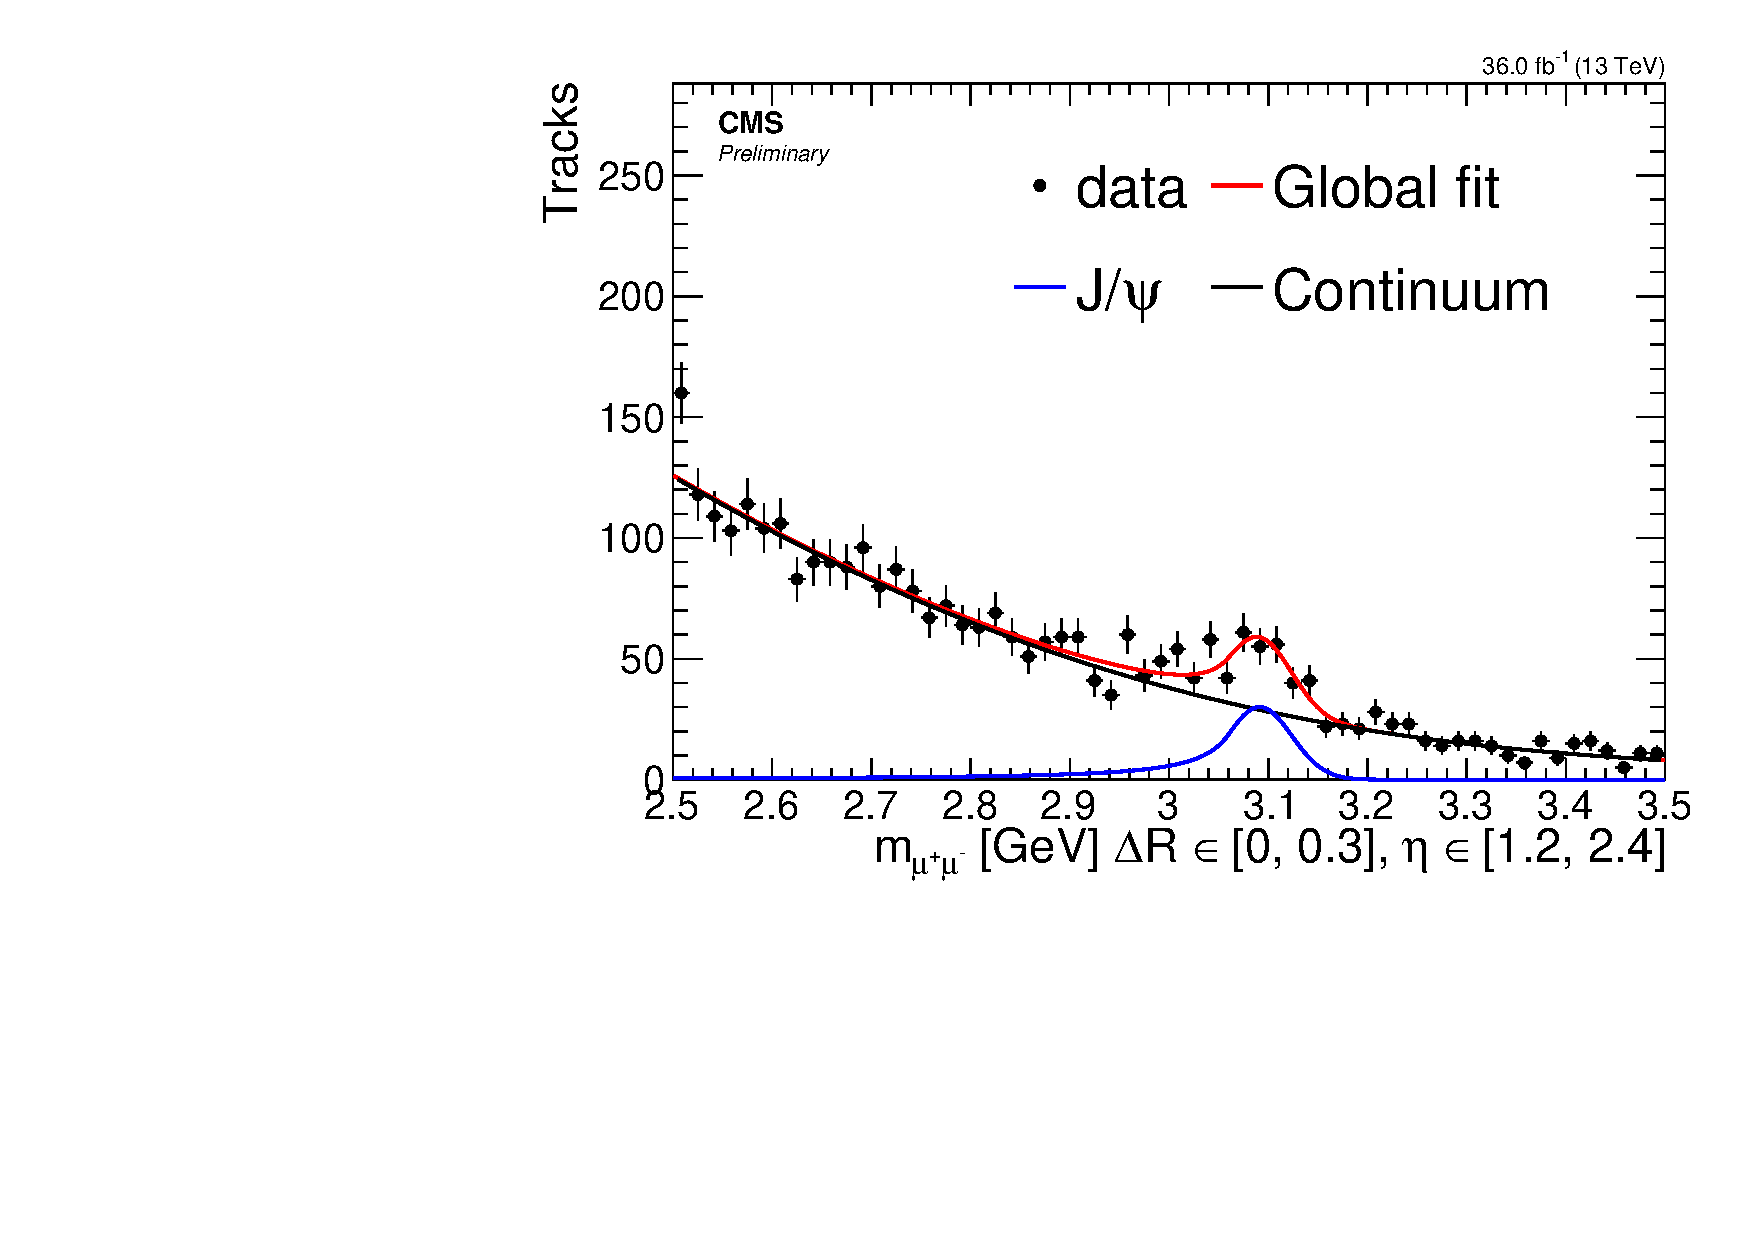
\includegraphics[width=0.32\linewidth]{plots/jpsi_muons_fit_data_delta_r_single_electron/none_invMass_0_0.3_1.2_2.4.pdf} \,
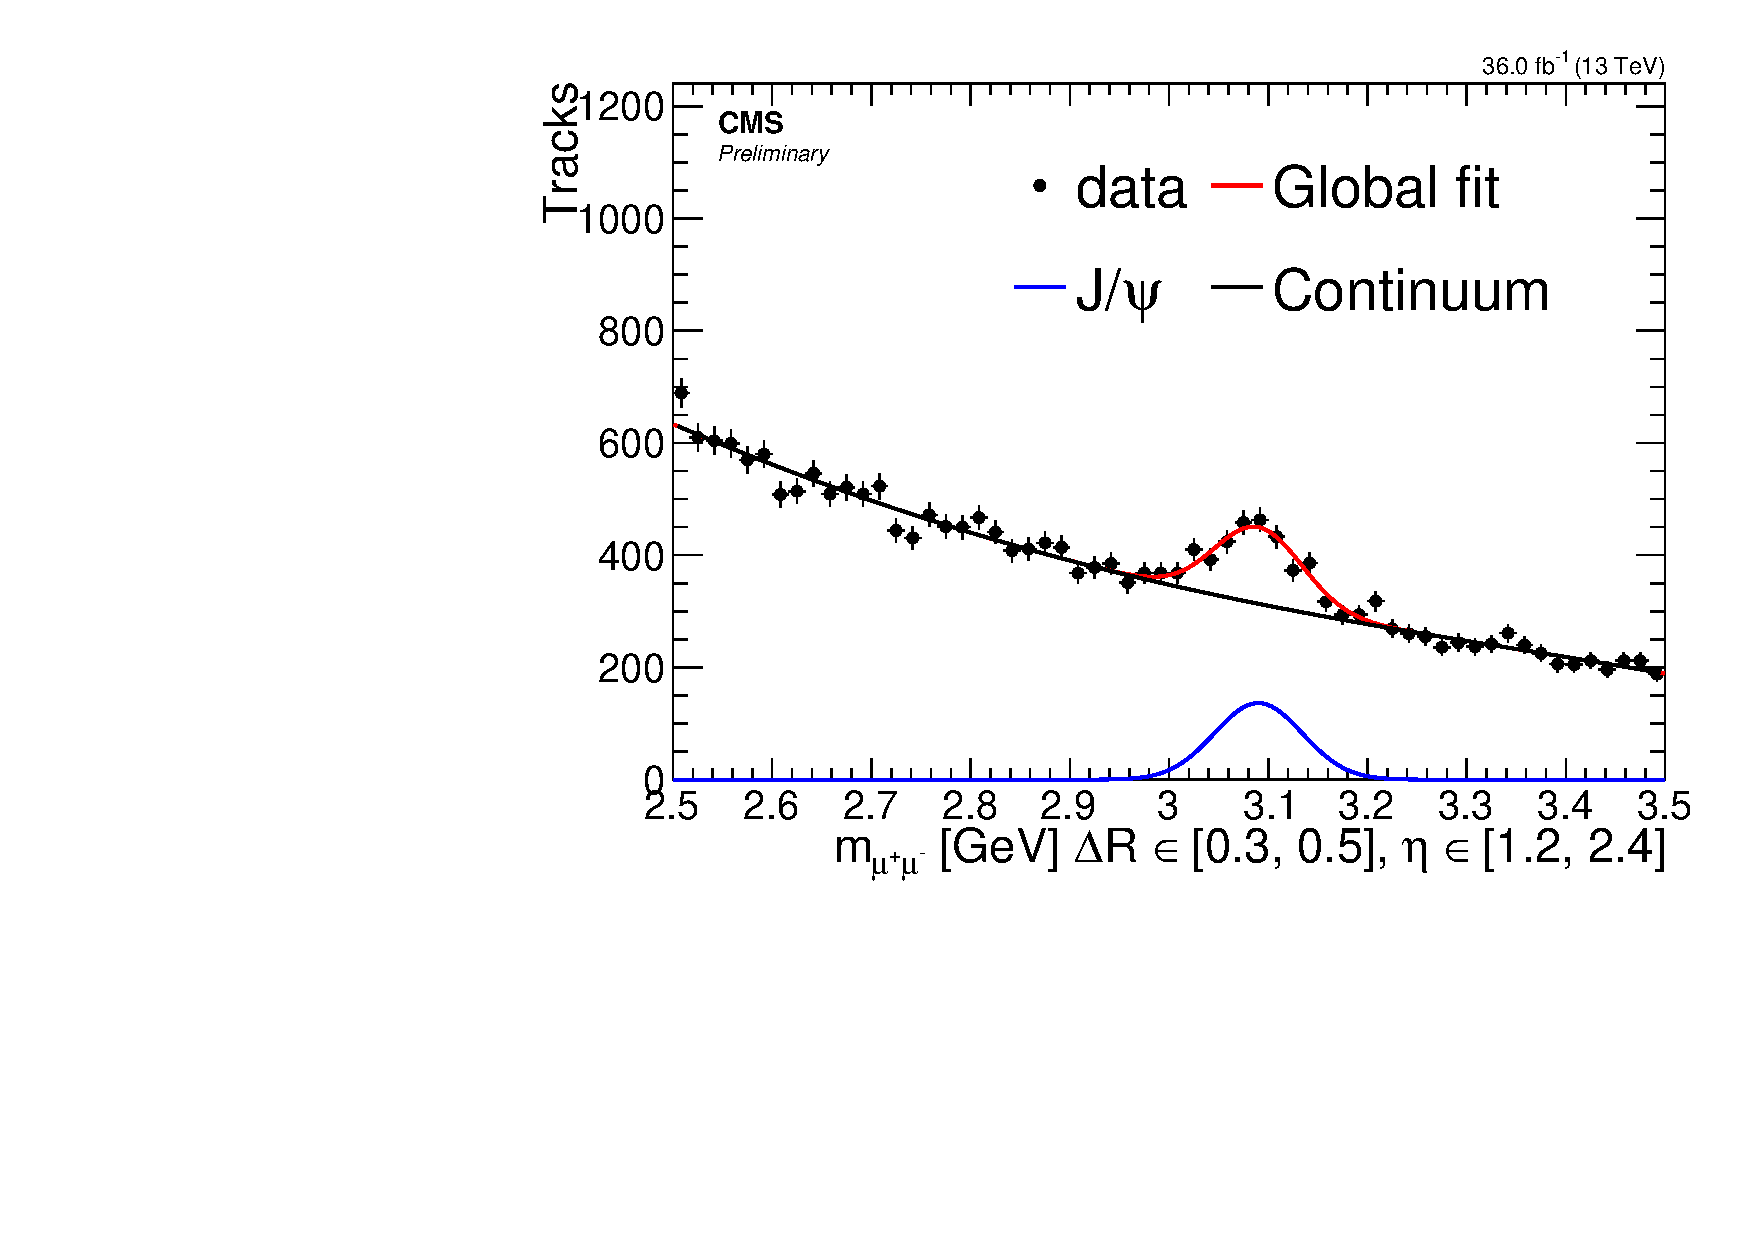
\includegraphics[width=0.32\linewidth]{plots/jpsi_muons_fit_data_delta_r_single_electron/none_invMass_0.3_0.5_1.2_2.4.pdf} \,
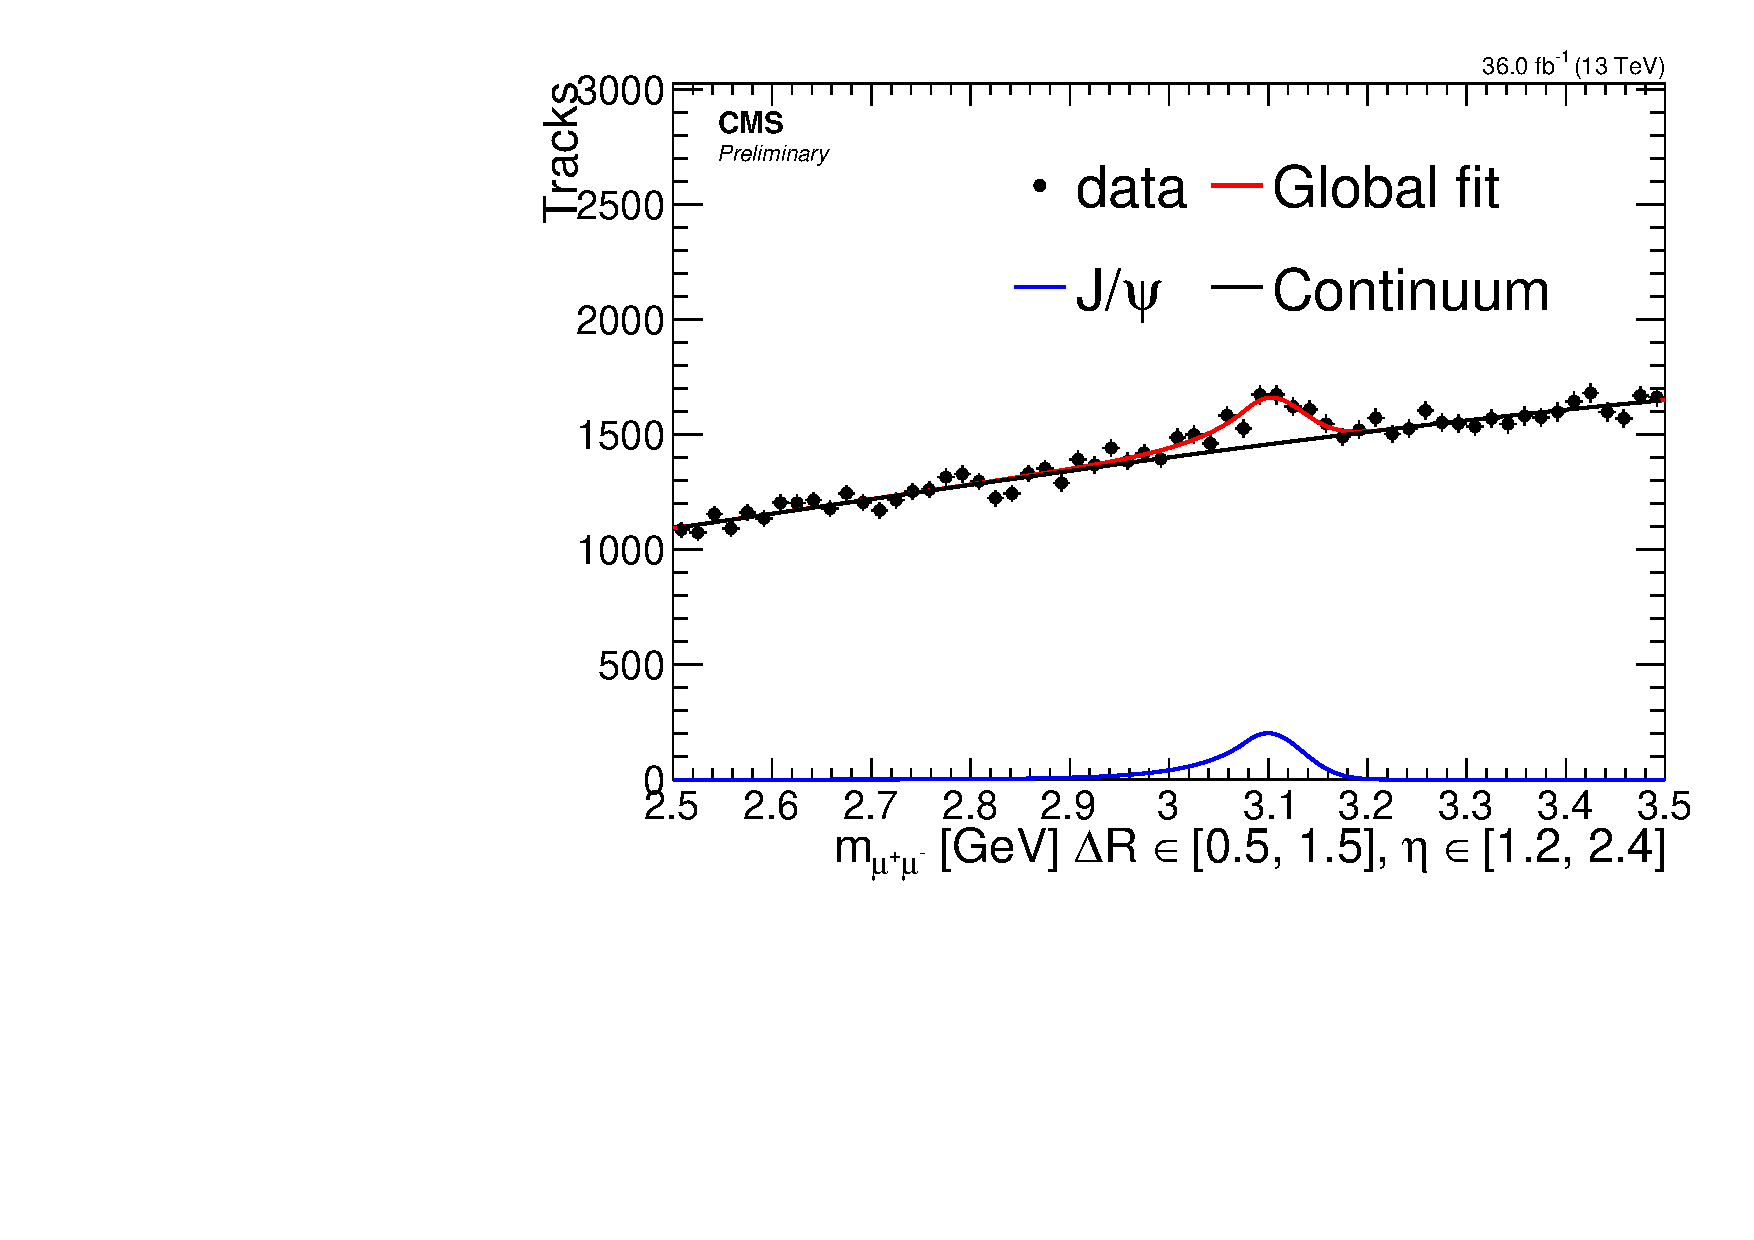
\includegraphics[width=0.32\linewidth]{plots/jpsi_muons_fit_data_delta_r_single_electron/none_invMass_0.5_1.5_1.2_2.4.pdf} \\
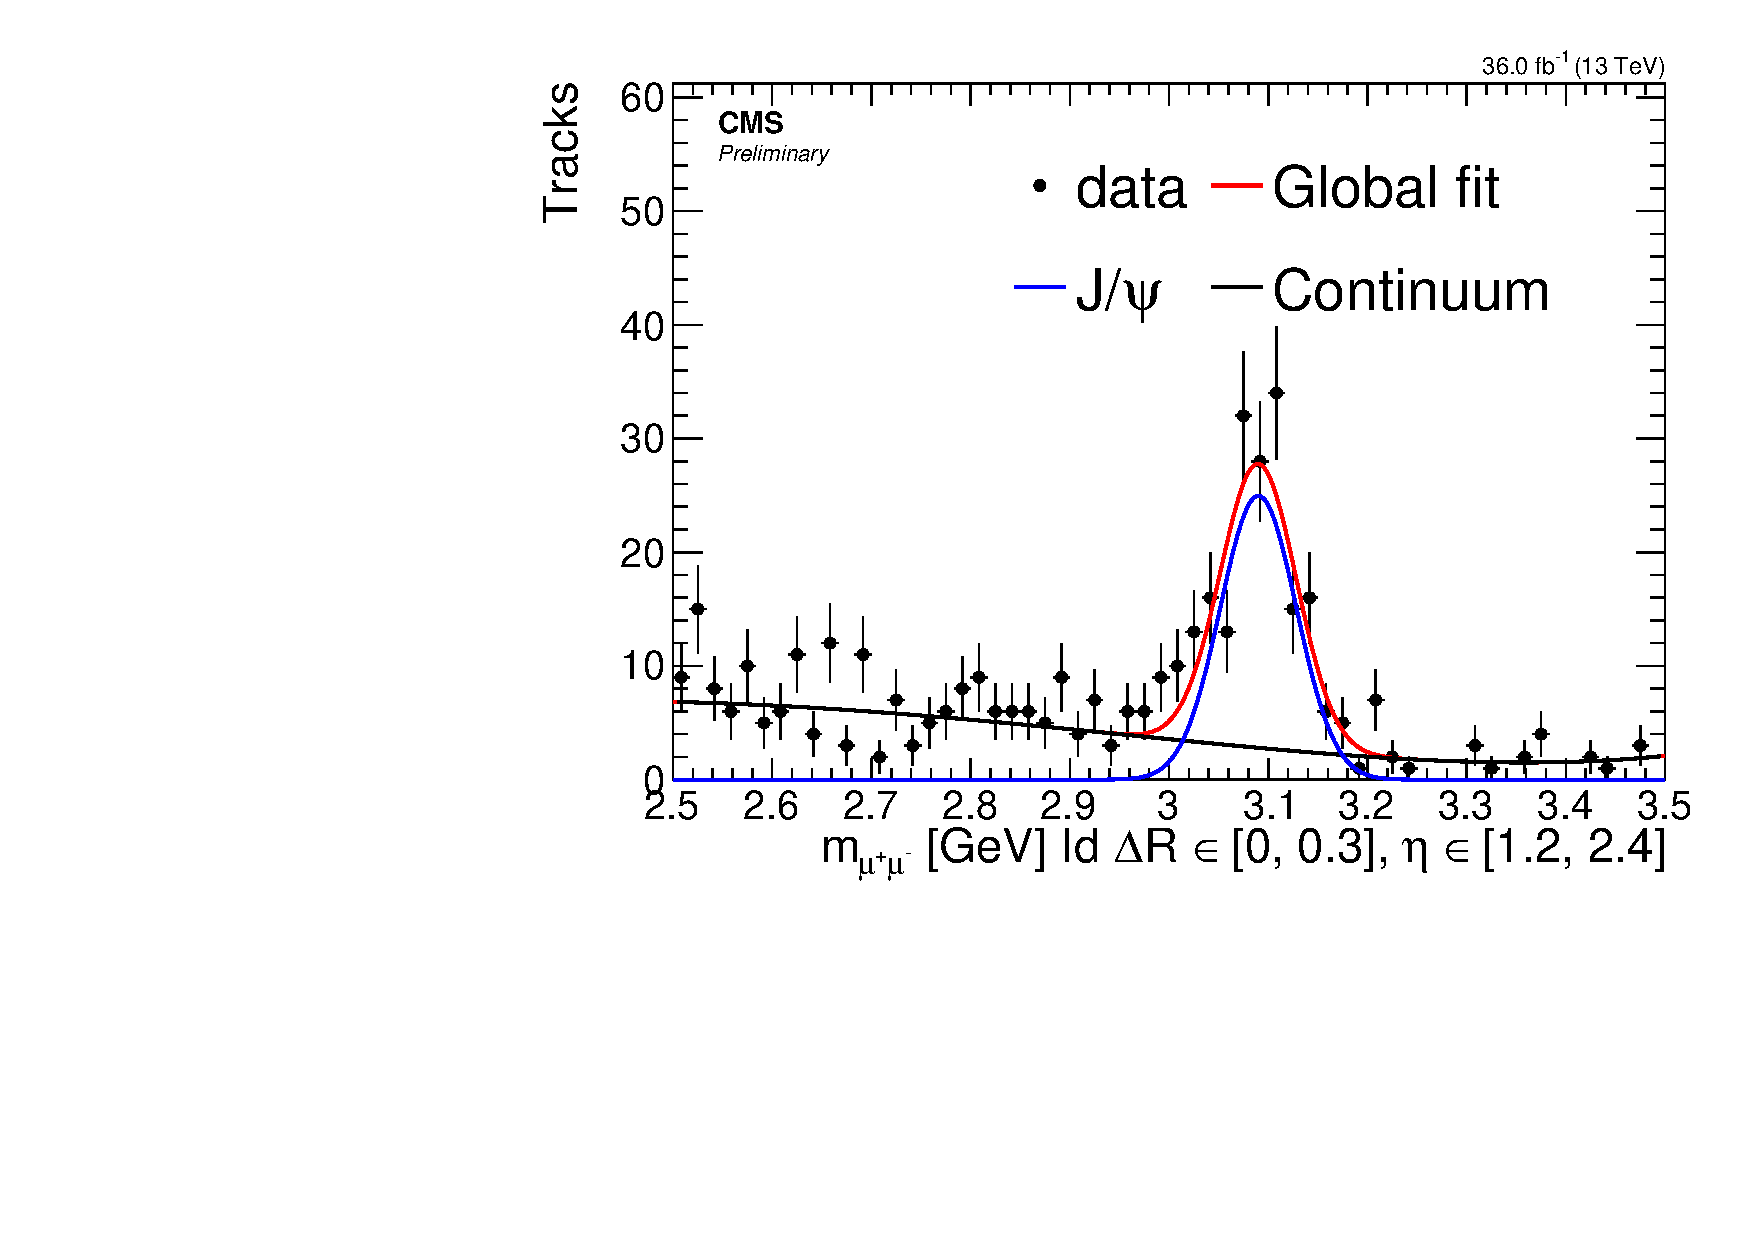
\includegraphics[width=0.32\linewidth]{plots/jpsi_muons_fit_data_delta_r_single_electron/none_id_invMass_0_0.3_1.2_2.4.pdf} \,
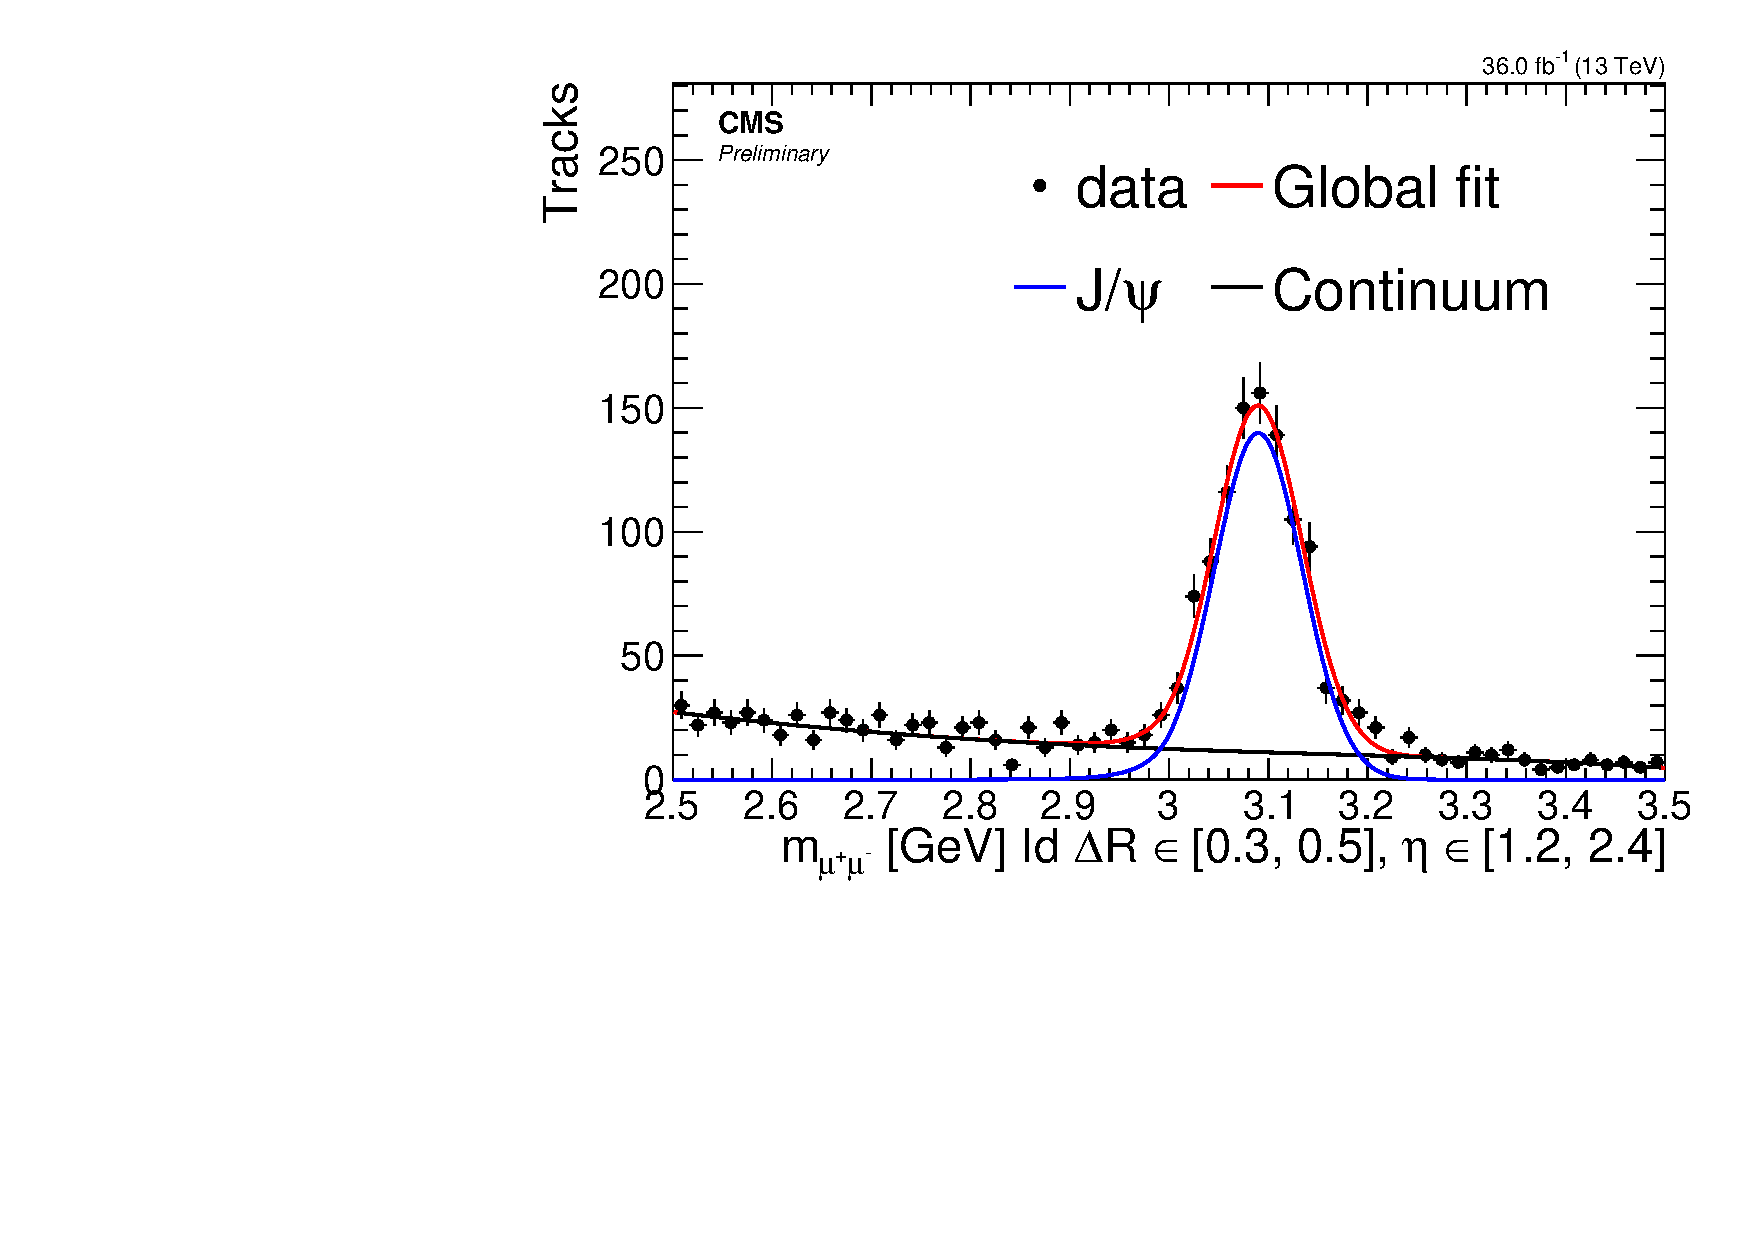
\includegraphics[width=0.32\linewidth]{plots/jpsi_muons_fit_data_delta_r_single_electron/none_id_invMass_0.3_0.5_1.2_2.4.pdf} \,
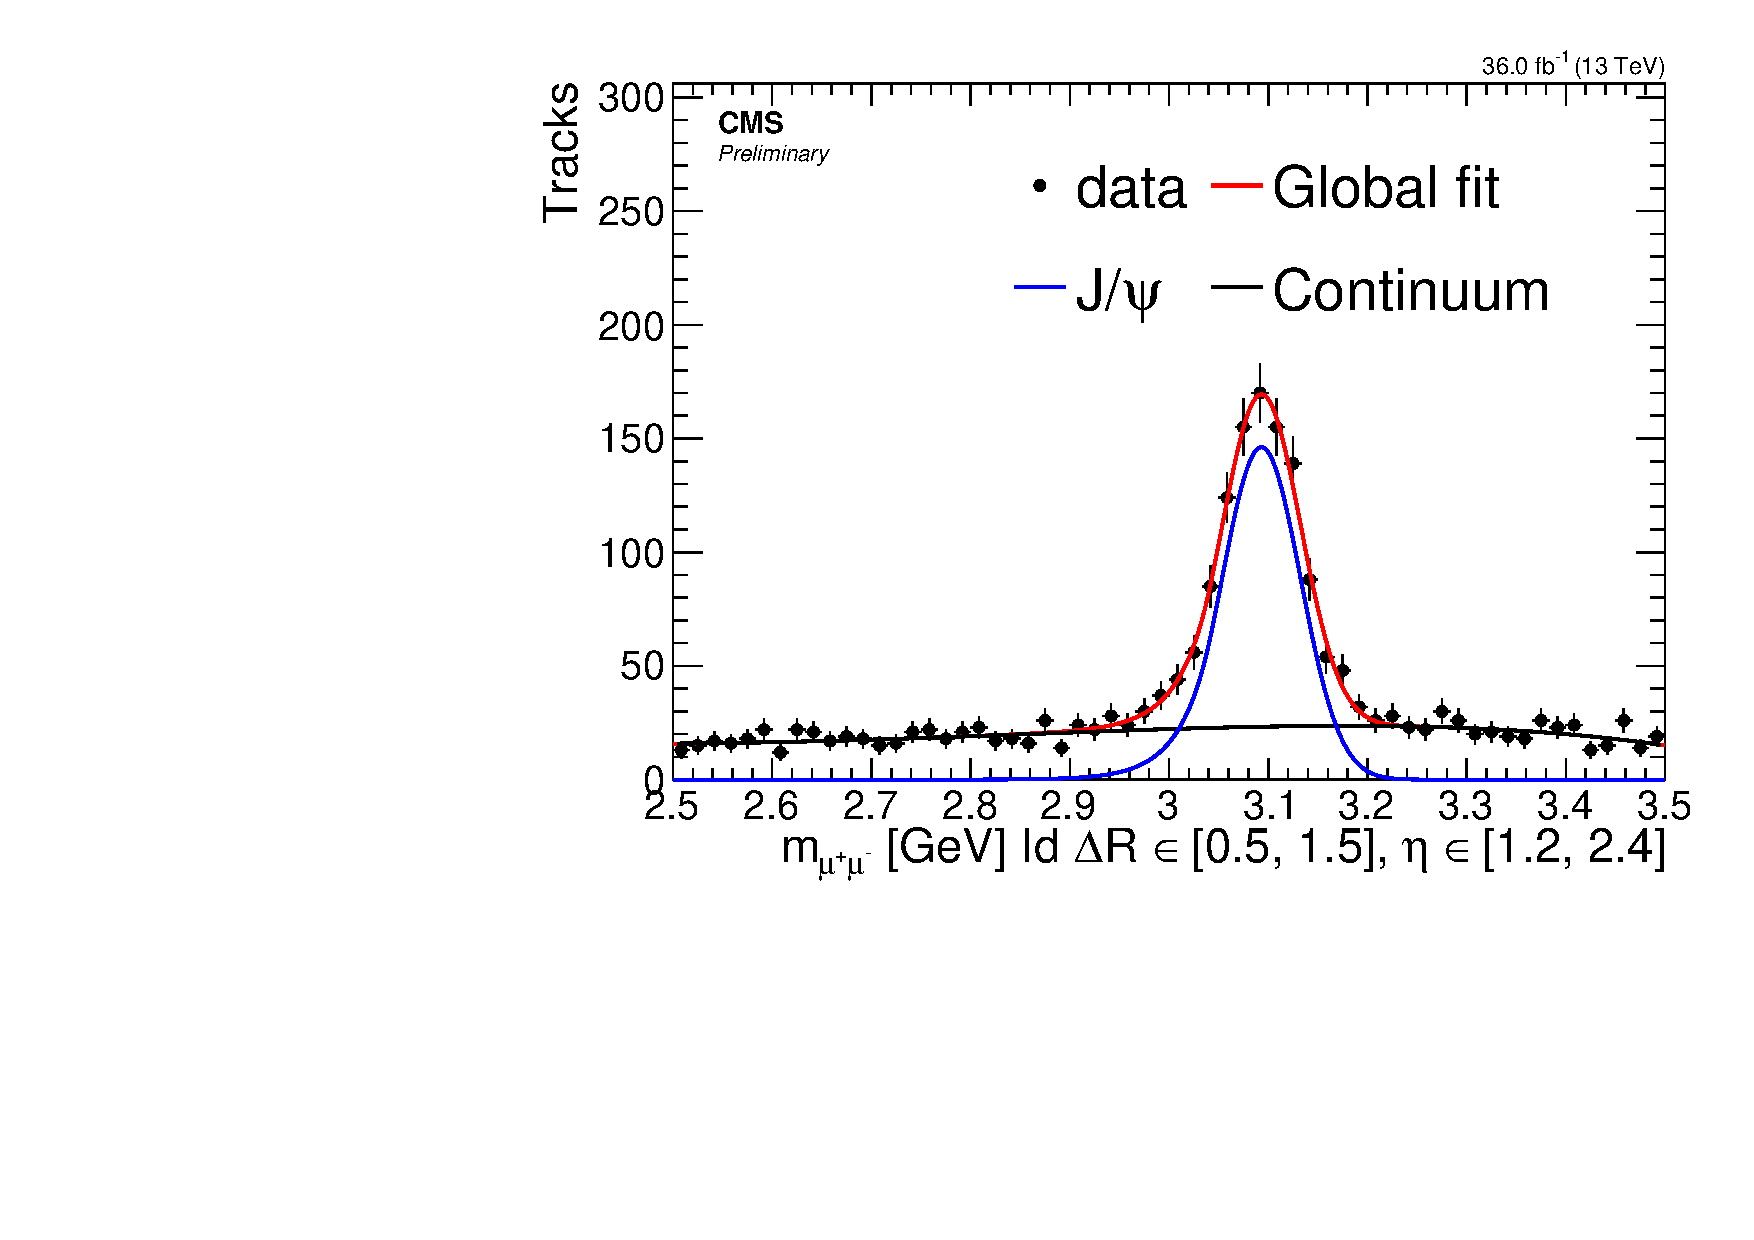
\includegraphics[width=0.32\linewidth]{plots/jpsi_muons_fit_data_delta_r_single_electron/none_id_invMass_0.5_1.5_1.2_2.4.pdf}  \\
\caption[Data endcaps muons fits]{Data endcaps muons fits for denominator (top) and numerator (bottom) for $0<\DR<0.3$  (left), $0.3<\DR<0.5$ (center), $0.5<\DR<1.5$ (right)}
\label{fig:tb-endcaps-data}
\end{figure}

The efficiencies and corresponding scale factors can be seen in Figure~\ref{fig:tb-eff-sf}. The scale factors are statistically consistent with unity and show no discernible $\DR$ dependence. A similar study was carried out with simulation and data for 2017 and 2018 in~\cite{muon-id-sf-2017-8}, and no $\DR$ dependence was observed either. As a result of these studies, the recommendation from the \gls{pog} is to use the calculated scale factors provided by them with an additional systematic uncertainty of 1\% for muons with $\pt<20\GeV$.

\begin{figure}[!htbp]
\centering
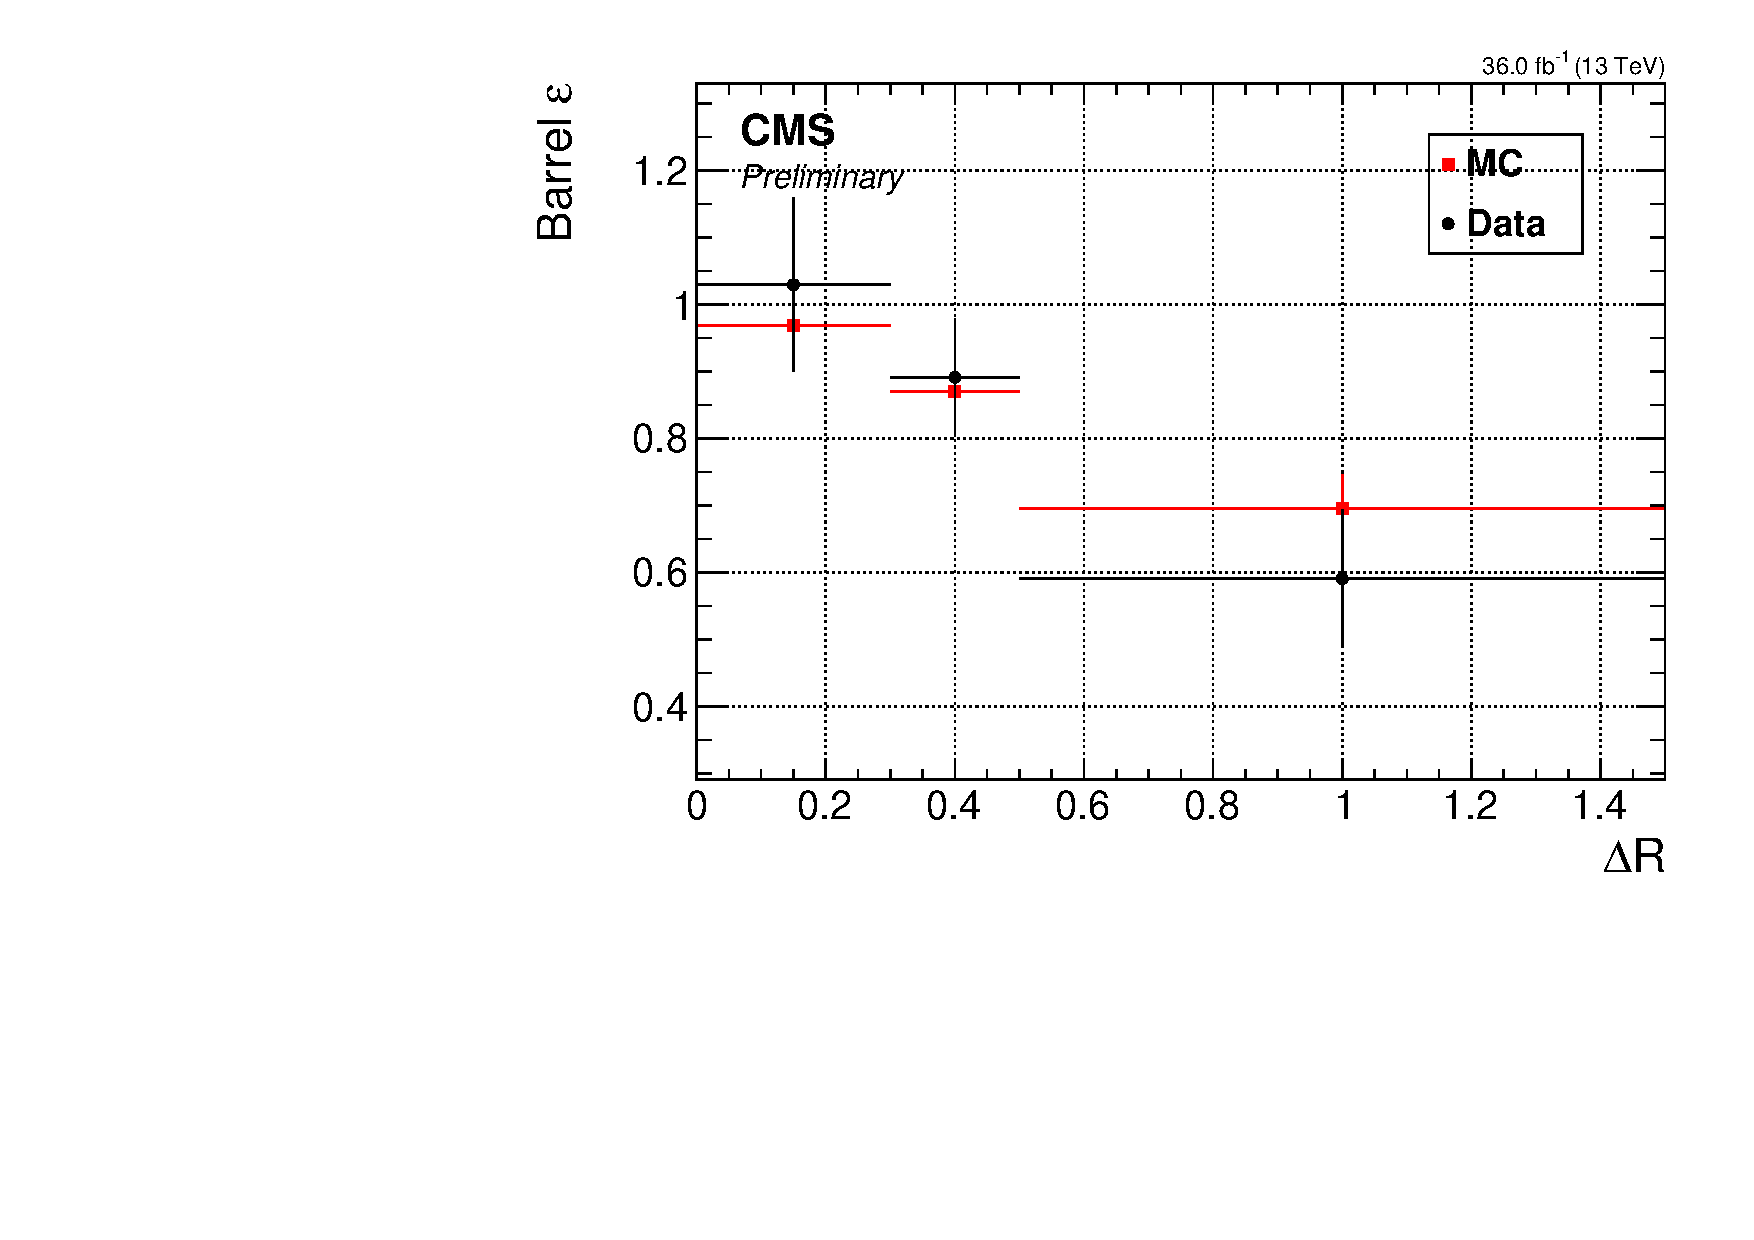
\includegraphics[width=0.48\linewidth]{plots/scale_factors/barrelDeltaRSingleElectron.pdf} \,
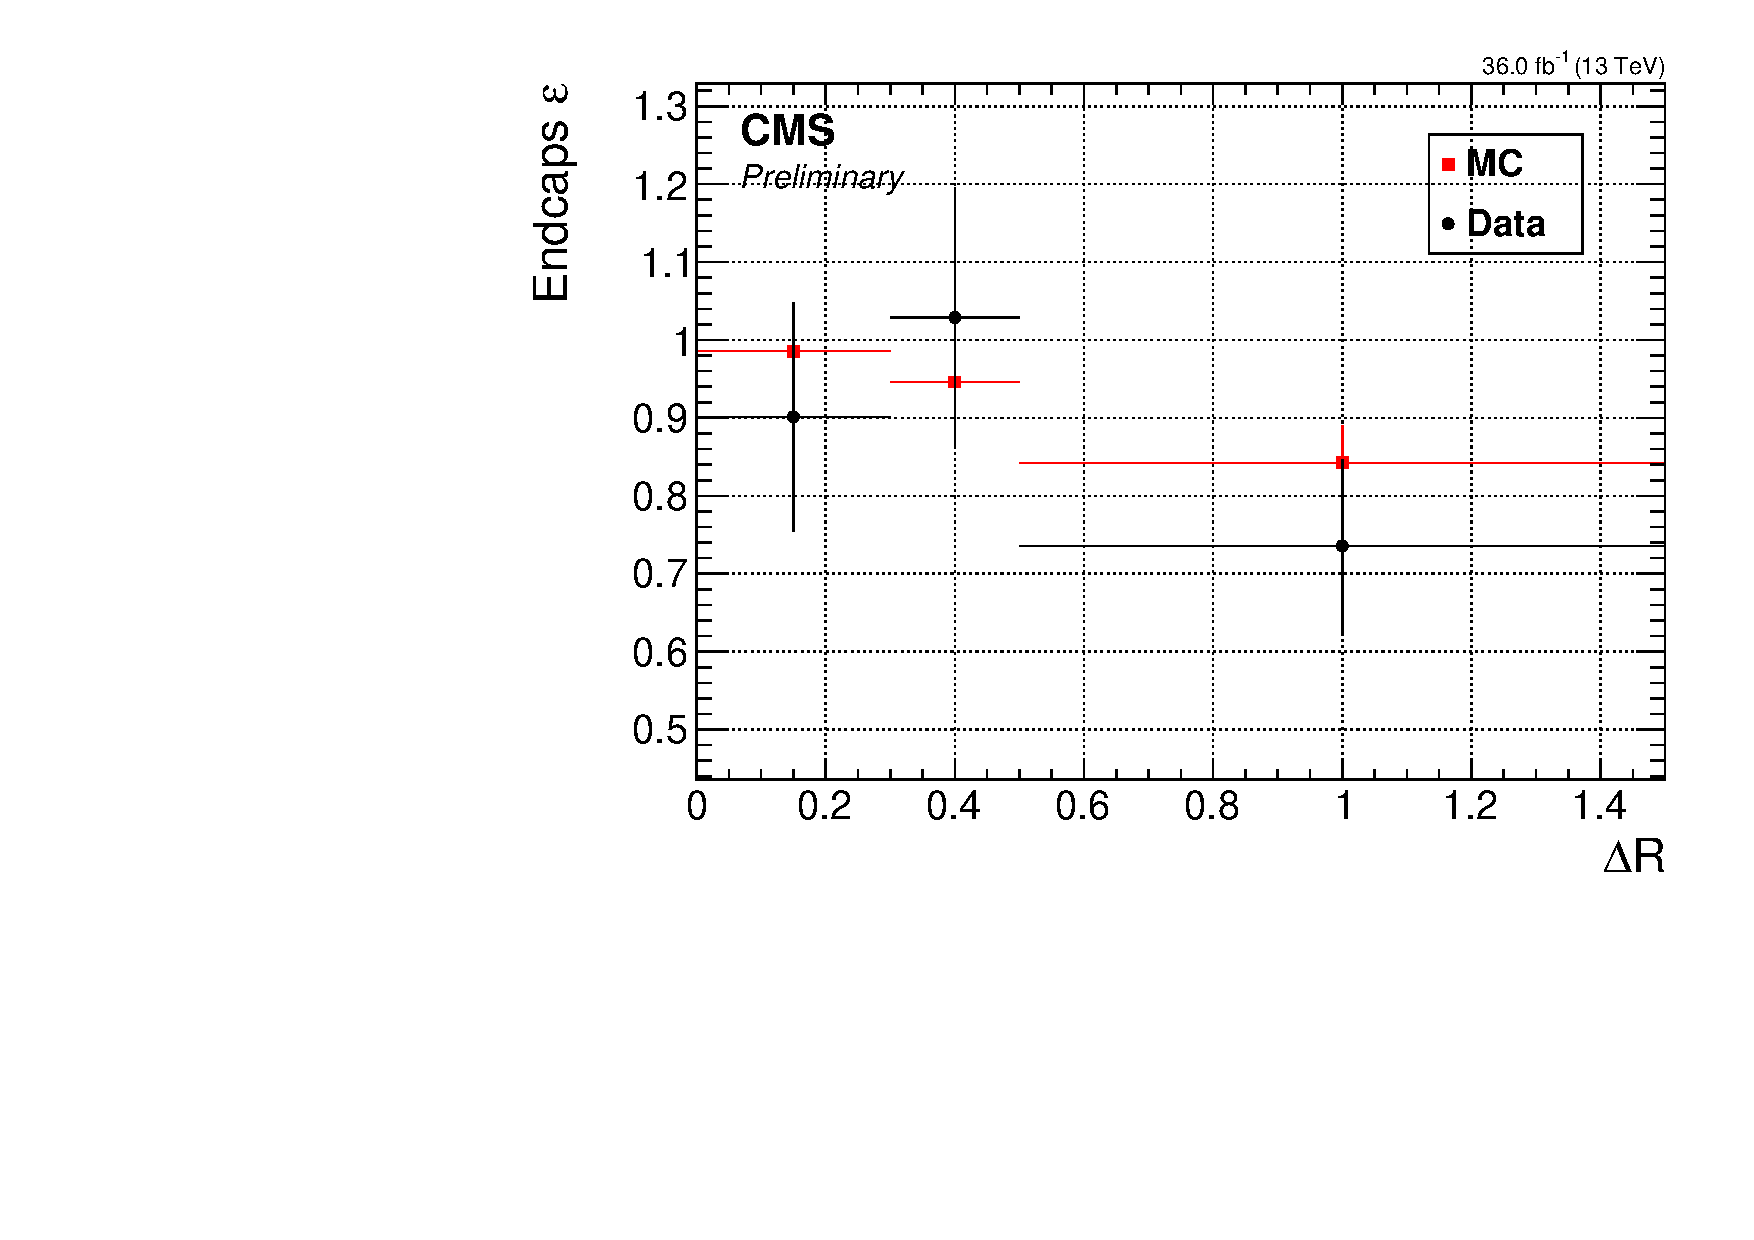
\includegraphics[width=0.48\linewidth]{plots/scale_factors/endcapsDeltaRSingleElectron.pdf}  \\
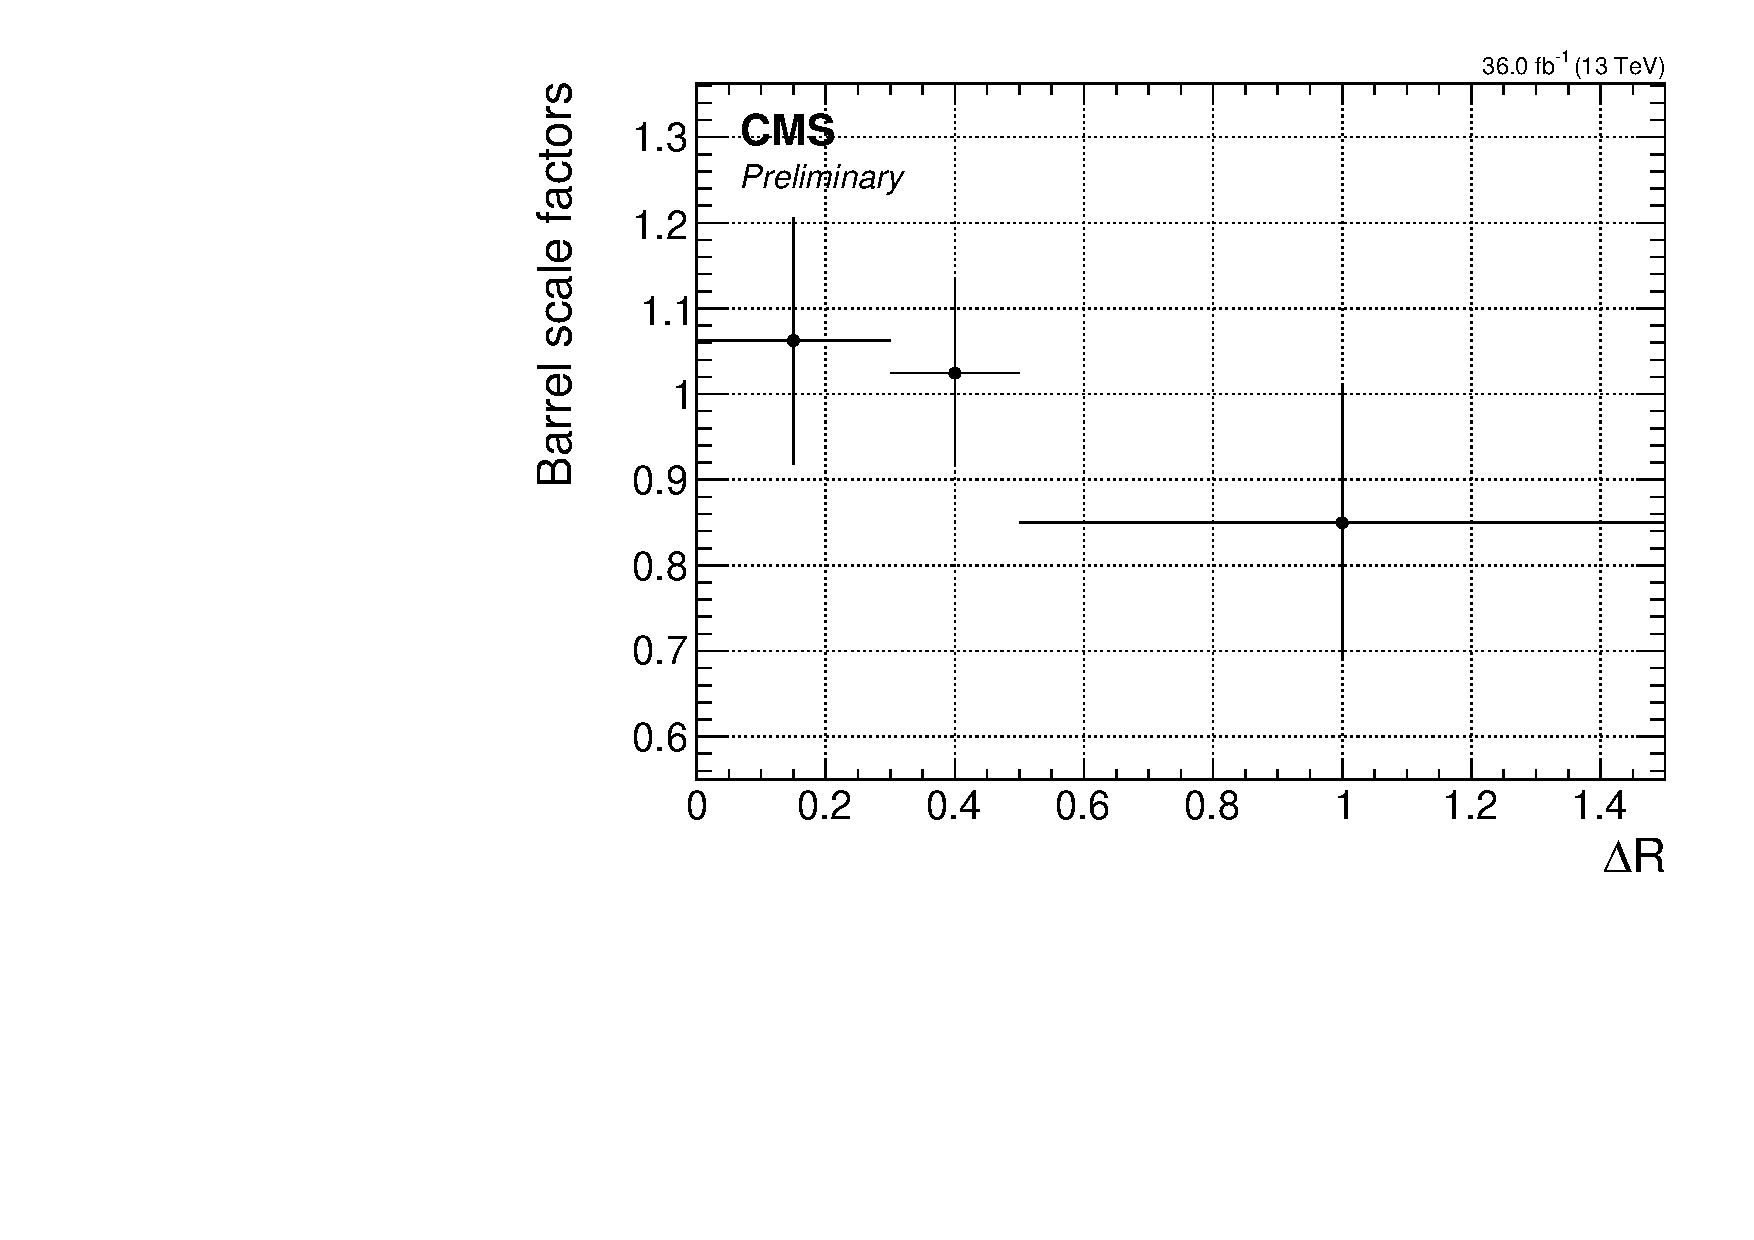
\includegraphics[width=0.48\linewidth]{plots/scale_factors/barrelDeltaRisoScaleFactorsSingleElectron.pdf} \,
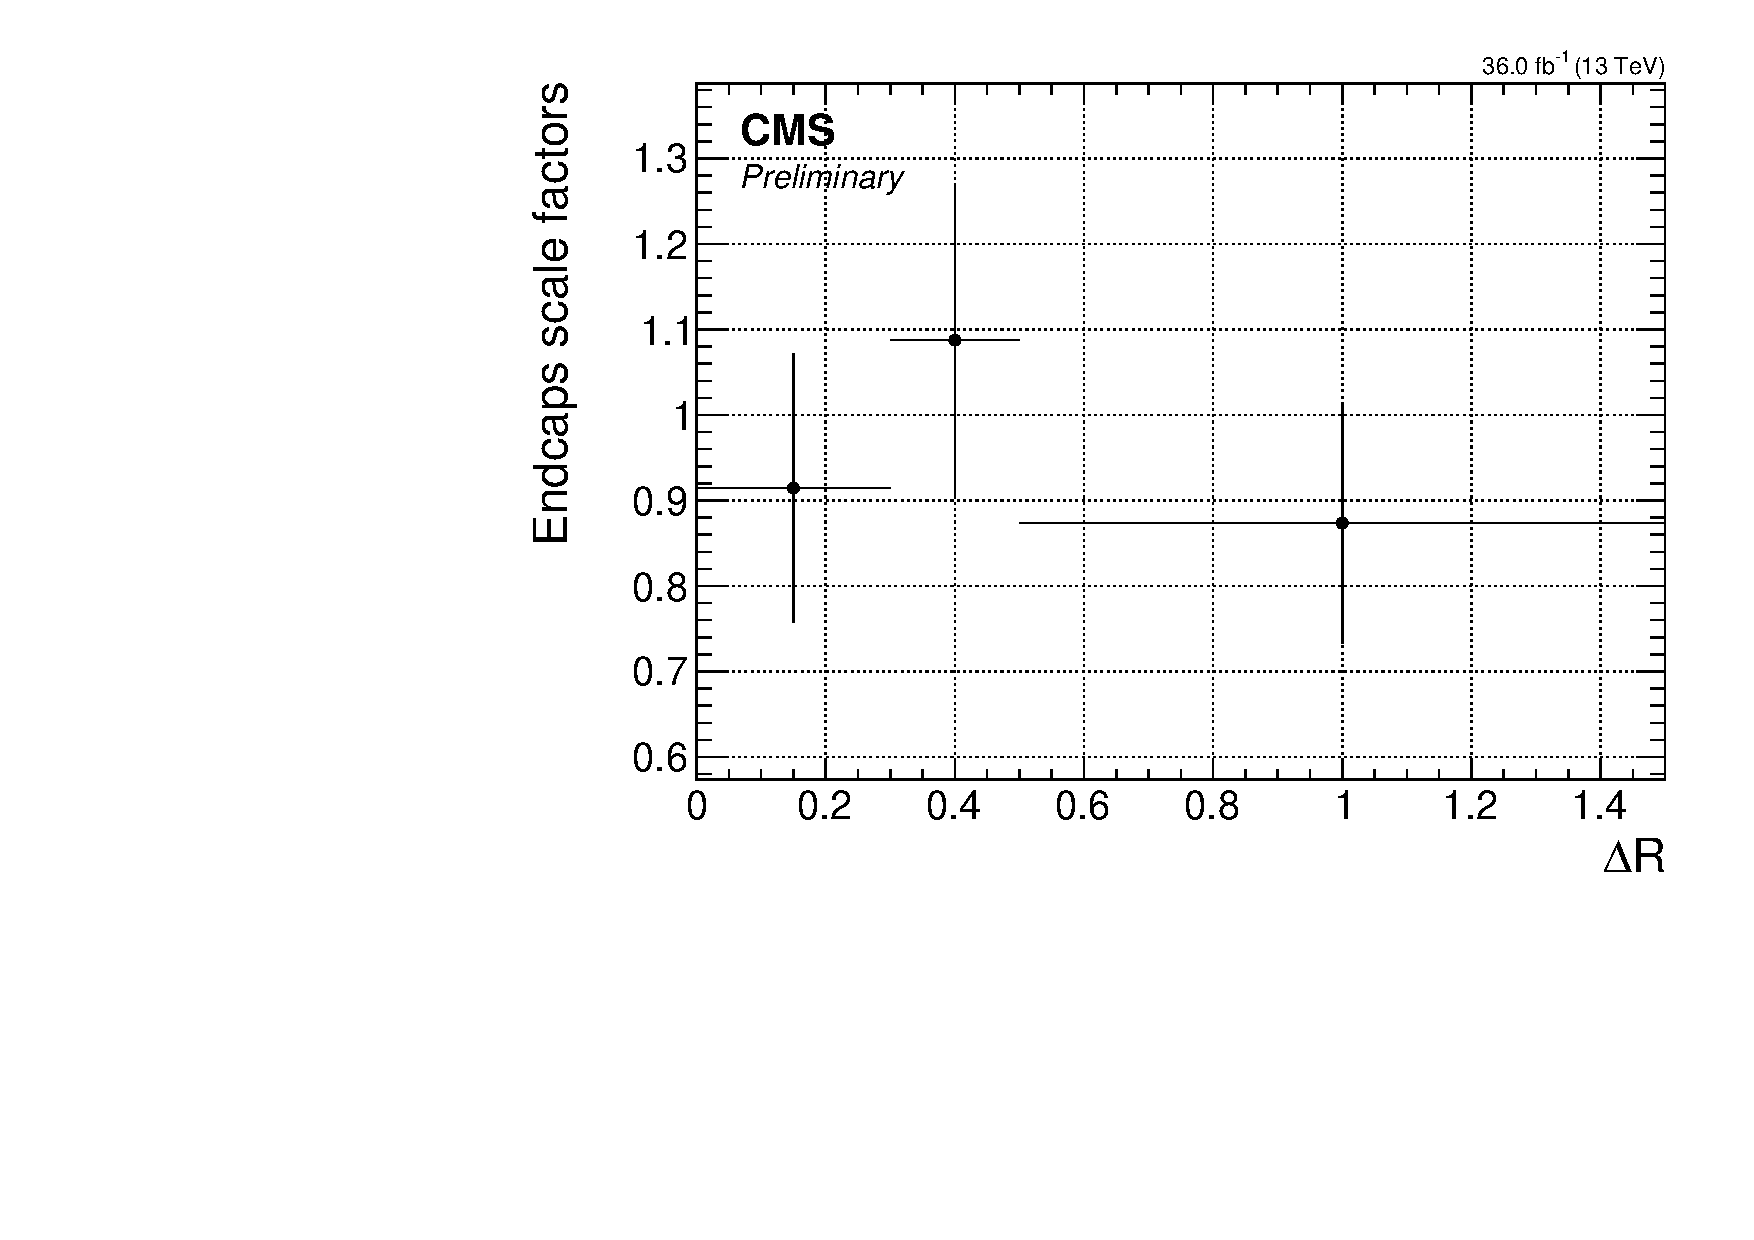
\includegraphics[width=0.48\linewidth]{plots/scale_factors/endcapsDeltaRisoScaleFactorsSingleElectron.pdf} \\
\caption[Efficiencies and scale factors]{Efficiencies (top) and scale factors (bottom) for barrel muons (left) and endcaps muons (right).}
\label{fig:tb-eff-sf}
\end{figure}